
In this section, we prove that \outofk Approximate \Sperner (without symmetry constraints) is \PPAD-complete. 
This is a warm-up proof for the \PPAD-completeness of the \outofk Approximate Symmetric \Sperner problem, whose hard instances and proof of \PPAD-completeness will be presented in the next section.
For convenience, we will not consider the query complexity in this warm-up section. 

\begin{theorem}
    For any constant $\delta>0$ and any $k=\poly(n)$, \outofk Approximate \Sperner is \PPAD-complete.
    In particular, there is a reduction in $\poly(n,k)$ time that reduces a 2{\rm D}-\Sperner instance with triangulation side-length of $2^n$ to a \outofk Approximate \Sperner instance with triangulation side-length of $2^{-3kn}$.
\end{theorem}

Because the \outofk Approximate \Sperner problem is a relaxation of $k${\rm D}-\Sperner problem, which is in \PPAD. 
The {\PPAD\xspace} membership of \outofk Approximate \Sperner problem is clear. 
Our focus of this section is to prove its \PPAD-hardness.

We will now begin describing our formal construction (still for the warm-up result). To help the reader keep track of the notation, both here and the main construction in the next section, we provide a summary in \cref{table:notation}.
%We present all our notations used in our proof in advance.
%\Ruiquan{I don't know where should we put this section}
% \Ruiquan{Also, I am not sure if I am missing some important notations.}

\begin{table}[h] 
\caption{Table of notation for Sections~\ref{sec:warmup-proof-for-approx-sperner} and~\ref{sec:final-proof-for-approx-sperner}}
    \centering
    \begin{tabular}{c|c|c} 
        \hline
        \hline
        {\bf \large Notation} & {\bf \large Description} & {\bf \large References} \\
        \hline
        \hline
        $\vec{x}$ & vectors (also, as $\vec{x'}, \vec{x}^{(1)}, \vec{x}^{(2)}, \dots$) & all sections\\
        $x_i$ & coordinates in vectors (also, as $x'_i, x^{(1)}_i, x^{(2)}_i, \dots$) & all sections\\
        $\Delta^k$ & standard $k$-simplex & \cref{def:standard-simplex}\\
        $\Delta_n^k$ & discrete $k$-simplex with a triangulation side-length of $2^{-n}$ & \cref{def:discrete-simplex}\\
        $C_{\rect}(\cdot)$ & 2{\rm D}-\rect\Sperner instances & \cref{def:rect-sperner}\\
        $C(\cdot)$ & base 2{\rm D}-\Sperner instances & \cref{alg:base-instance}\\
        $C^{(k)}(\cdot)$ & \outofk Approximate \Sperner instances & \cref{alg:base-instance,alg:approx-sperner-kgeq3}\\
        $C^{(k)}_{\rm sym}(\cdot)$ & \outofk Approximate Symmetric \Sperner instances & \cref{alg:approx-symmetric-sperner-kgeq3} \\
        $\alpha(\cdot)$ & shrinking factor & \cref{eqn:shrinking-factor}\\
        $\rel(\cdot)$ & coordinate converter & \cref{eqn:coordinate-converter} \\
        $\rela(\cdot)$ & coordinate converter for symmetry & \cref{eqn:new-coordinate-converter}\\
        $d(\cdot,\cdot)$ & a metric to define $\rel$ & \cref{eqn:modified-distance}\\
        $d^{\alpha}(\cdot,\cdot)$ & an asymmetric quasimetric to define $\rela$ & \cref{eqn:shrinking-distance}\\
        $\nn(\cdot)$ & nearest neighbor & \cref{eqn:nn}\\
        $\nna(\cdot)$ &  nearest neighbor w.r.t. $\alpha$ & \cref{eqn:cnn-and-nn-for-symmetric}\\
        $\mathcal{N}(\cdot)$ & neighborhood of size $\eps\times \eps$ & \cref{def:neighbourhood} \\
        $C_{\sf nn}(\cdot)$ & neighboring color (i.e., the color of the nearest neighbor) & \cref{eqn:cnn}\\
        $\hat{C}_{\sf nn}(\cdot)$ & the modified neighboring color & \cref{eqn:modified-neighboring-color}\\
        $C_{\sf nn}^{\alpha}(\cdot)$ &  the neighboring color w.r.t. $\alpha$ & \cref{eqn:cnn-and-nn-for-symmetric}\\
        $\hat{C}_{\sf nn}^{\alpha}(\cdot)$ &  the modified neighboring color w.r.t. $\alpha$ & \cref{eqn:modified-neighboring-color-symmetry}\\
        $\sim_C$ & symmetry in colorings (binary relation) & \cref{def:symmetry-in-coloring} \\
        $\simrel$ & equivalence between converted coordinates (binary relation) & \cref{def:equiv-converted-coordinates}\\
        $\vec{P}(\cdot)$ & the projection step from $\Delta^{k}$ to $\Delta^{k-1}$ (for any $k$) & \cref{def:projection}\\
        $\vec{P}^{(\ell)}(\cdot)$ & performing $\ell$ projection steps & \cref{def:lth-projection}\\
        $i^*(\cdot)$ & the index of the first non-zero entry & \cref{eqn:first-nonzero-index}\\
        $\vec{y}^{(i)}(\cdot)$ & the $i$-th intermediate projection (\cref{subsec:symmetric-kd,,subsec:warmup-kd} only) & \cref{alg:approx-sperner-kgeq3,,alg:approx-symmetric-sperner-kgeq3} \\
        $\vec{c}^{(i)}(\cdot)$ & the $i$-th intermediate palette (\cref{subsec:symmetric-kd,,subsec:warmup-kd} only) & \cref{alg:approx-sperner-kgeq3,,alg:approx-symmetric-sperner-kgeq3} \\
        % TBC & TBC & TBC \\
        \hline
    \end{tabular} \label{table:notation}
\end{table}

We will construct a chain of \PPAD-hard instances $C^{(2)}, C^{(3)}, \dots$ to prove this warm-up technical result. 
We will present the first instance of the chain $C^{(2)}$ in \cref{subsec:warmup-2d}.
Later, this $C^{(2)}$ will also serve as the base \PPAD-hard 2{\rm D}-\Sperner instance $C$ (i.e., we will use the notation $C$ when referring to the base instance), and we will present in \cref{subsec:warmup-kd} a recursive way that constructs $C^{(k+1)}$ by combining $C^{(k)}$ with one copy of this base 2{\rm D}-\Sperner instance $C$. 
Towards this end, in \cref{subsec:warmup-convert} we introduce an intermediate function, which we call the {\em coordinate converter}; this function projects points in a standard $2$-simplex to real values in $[0,1]$ (the {\em converted coordinate}). When we move from $C^{(k)}$ to $C^{(k+1)}$ we have a new coordinate; we embed a copy of the base instance $C$ on the plane spanned by the new coordinate and the converted coordinate. 

Our instances will be constructed in continuous space instead of discrete space. 
That is, our \outofk Approximate \Sperner instance is a function $C^{(k)}: \Delta^{k} \to [k+1]$ satisfying the following hardness result.
For simplicity, we define $\eps\defeq 2^{-n}$ and will use $\eps$ and $2^{-n}$ interchangeably. 
\begin{theorem}
    \label{thm:continuous-asymmetry-main}
    There exists a chain of functions $\{C^{(k)}: \Delta^k \to [k+1]\}_{k\geq 2}$ that can be computed in $\poly(|\vec{x}|)$ time for each $\vec{x}\in \Delta^k$, where $|\vec{x}|$ is the bit complexity of $\vec{x}$ and satisfies the following property. 
    For any $k\geq 2$, it is \PPAD-hard to find three points $\vec{x}^{(1)}, \vec{x}^{(2)}, \vec{x}^{(3)}\in \Delta^{k}$ such that 
    \begin{itemize}[itemsep=0.2em, topsep=0.5em]
        \item {\bf they are close enough to each other:} for any $i,j\in [3]$, $\normtxt{\vec{x}^{(i)}-\vec{x}^{(j)}}{\infty}\leq 2^{-3kn}=\eps^{3k}$, 
        \item {\bf they induce a trichromatic triangle:} $|\settxt{C^{(k)}(\vec{x}^{(i)}):i\in [3]}|=3$. 
    \end{itemize}
\end{theorem}

\subsection{Hard instances with two dimensions}
\label{subsec:warmup-2d}
In this subsection, we will present a family of continuous $2${\rm D}-\Sperner instances that will serve both as the base \PPAD-complete instance we will embed into this chain of \outofk Approximate \Sperner instances and as the second instance $C^{(2)}$ in the chain.
Note that for $k=2$, the \outofk Approximate \Sperner problem is equivalent to the $2${\rm D}-\Sperner problem (\cref{remark:equiv-at-2}).

\paragraph{The instances.} This family of instances is constructed based on the hard instances of \textcite{DBLP:journals/tcs/ChenD09}.
They first construct a core rectangle which has a  boundary condition similar to $2$D-\Sperner, and show that it is \PPAD-hard to find a small trichromatic triangle in the core rectangle. 
In particular, their paper can easily imply that the following rectangular version of the 2D-\Sperner problem\footnote{In the original paper of \textcite{DBLP:journals/tcs/ChenD09}, they name this rectangular version as $2$D-\Brouwer.} is \PPAD-complete. 
\begin{definition}[2{\rm D}-\rect\Sperner]
    \label{def:rect-sperner}
    Let $Q^2_n = \{0,1,\dots,2^n-1\}^2$ denote the 2D grid with side-length of $2^n$ on each dimension. 
    In $2${\rm D}-\rect\Sperner, we are given coloring $C:Q^2_n \to [3]$ satisfying: (1) $C(x,0)\in \{1,2\}$ and $C(x,2^{n}-1)=3$ for any $x\in Q_n$; and (2) $C(0,0)=1, C(2^n-1,0)=2$, and $C(0,y)=C(2^{n}-1,y)=3$ for any $y\in Q_n\setminus \{0\}$. 
    The goal of $2${\rm D}-\rect\Sperner is to find $\vec{x^*}\in ( Q_{n}\setminus \{2^n-1\}  )^2$ such that $|\settxt{C(\vec{x}): x_i \in \settxt{x_{i}^*,x_{i}^*+1} }|=3$.
\end{definition}

\begin{theorem}[\cite{DBLP:journals/tcs/ChenD09}]
    $2${\rm D}-\rect\Sperner is \PPAD-complete.
\end{theorem}
The way~\textcite{DBLP:journals/tcs/ChenD09} use this core rectangle is embedding it into a larger (triangular) $2${\rm D}-\Sperner instance, maintaining the \PPAD-hardness by filling the colors outside this rectangle without creating spurious trichromatic triangles. 
In this paper, we will continue to use this idea but with some slight modifications.
The first modification is that we turn the core rectangle into a continuous one, by mapping each point on the discrete 2D grid to a small square on a continuous 2D grid.
Formally, we map each point $(x,y)$ to the square $[\eps x, \eps(x+1))\times [\eps y,\eps (y+1))$. 
The second modification 
is that we embed this core rectangle in a small region 
inside the $2$-simplex and color for the remainder of the $2${\rm D}-\Sperner instance, ensuring that (1) the bottom $1$-simplex (points $\vec{x}\in \Delta^2$ with the third coordinate $x_3=0$) is equally colored by $1$ and $2$; 
(2) the other two boundaries of the 2-simplex (other than the base $1$-simplex) are colored symmetrically, i.e. $C(\vec{x})=3$ {\em iff} $x_3>0.1$.
\cref{alg:base-instance} and \cref{fig:continuous-mapping} conclude our embedding of the core rectangle inside a $2$-simplex.
We will call this part of the $2$-simplex the {\em core region}. 
\cref{lem:base-instance-bottom-slice,,lem:base-instance-lr-boundaries} conclude the aforementioned boundary conditions.
\cref{lem:base-instance-ppad-hard} establishes the computational complexity of the base instances. 

\begin{figure}[t]
    \centering
    
\tikzset{%
    every neuron/.style={
        circle,
        draw,
        minimum size=4pt,
        inner sep=0pt,
        very thin
    },
    neuron/.style={
        circle,
        fill=Purple,
        inner sep=0pt,
        minimum size=3.5pt
    },
}
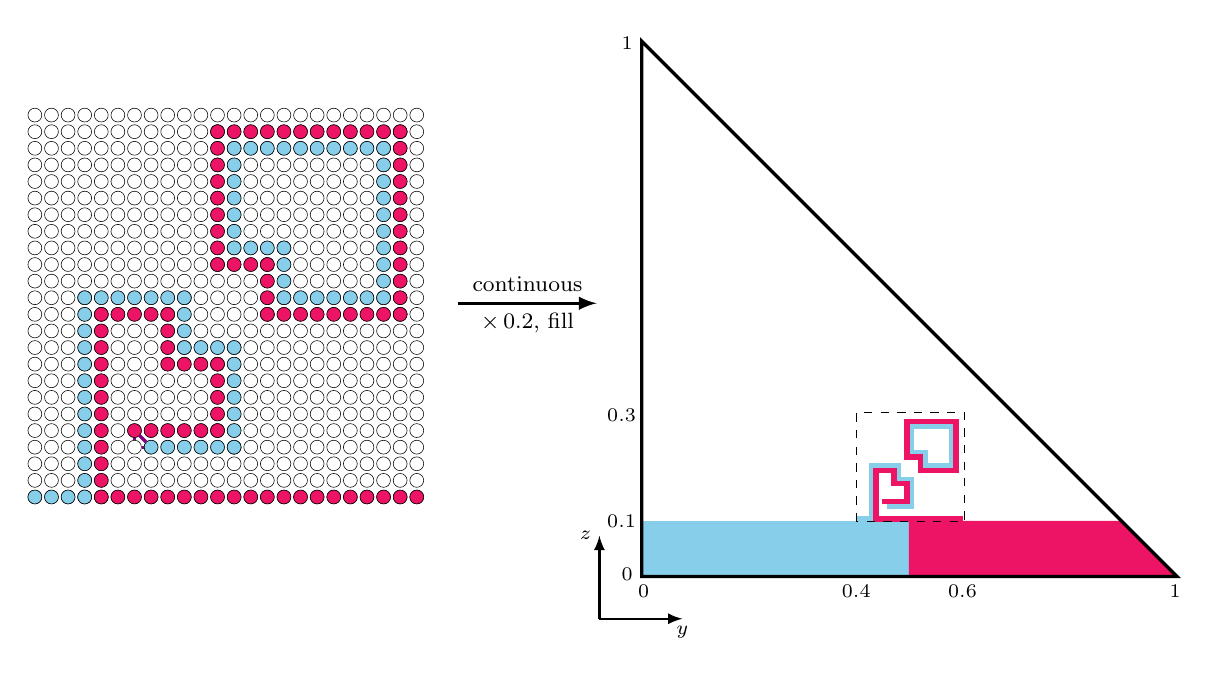
\begin{tikzpicture}[x=0.9cm, y=0.9cm, >=latex, every text node part/.style={align=center}]
    \foreach \x in {0,...,23}
        \foreach \y in {0,...,23} {
            \node [every neuron/.try] (f\x\y) at (6pt*\x+36pt,6pt*\y+24pt) {};
        } 
    \foreach \x in {0,...,3}
        \foreach \y in {0,...,0} {
            \node [every neuron/.try, fill=SkyBlue] (f\x\y) at (6pt*\x+36pt,6pt*\y+24pt) {};
        } 
    \foreach \x in {4,...,23}
        \foreach \y in {0,...,0} {
            \node [every neuron/.try, fill=WildStrawberry] (f\x\y) at (6pt*\x+36pt,6pt*\y+24pt) {};
        } 
    \foreach \x in {3,...,3}
        \foreach \y in {0,...,12} {
            \node [every neuron/.try, fill=SkyBlue] (f\x\y) at (6pt*\x+36pt,6pt*\y+24pt) {};
        } 
    \foreach \x in {4,...,4}
        \foreach \y in {0,...,11} {
            \node [every neuron/.try, fill=WildStrawberry] (f\x\y) at (6pt*\x+36pt,6pt*\y+24pt) {};
        } 
    \foreach \x in {3,...,9}
        \foreach \y in {12,...,12} {
            \node [every neuron/.try, fill=SkyBlue] (f\x\y) at (6pt*\x+36pt,6pt*\y+24pt) {};
        } 
    \foreach \x in {4,...,8}
        \foreach \y in {11,...,11} {
            \node [every neuron/.try, fill=WildStrawberry] (f\x\y) at (6pt*\x+36pt,6pt*\y+24pt) {};
        } 
    \foreach \x in {9,...,9}
        \foreach \y in {9,...,12} {
            \node [every neuron/.try, fill=SkyBlue] (f\x\y) at (6pt*\x+36pt,6pt*\y+24pt) {};
        } 
    \foreach \x in {8,...,8}
        \foreach \y in {9,...,11} {
            \node [every neuron/.try, fill=WildStrawberry] (f\x\y) at (6pt*\x+36pt,6pt*\y+24pt) {};
        } 
    \foreach \x in {9,...,12}
        \foreach \y in {9,...,9} {
            \node [every neuron/.try, fill=SkyBlue] (f\x\y) at (6pt*\x+36pt,6pt*\y+24pt) {};
        } 
    \foreach \x in {8,...,11}
        \foreach \y in {8,...,8} {
            \node [every neuron/.try, fill=WildStrawberry] (f\x\y) at (6pt*\x+36pt,6pt*\y+24pt) {};
        } 
    \foreach \x in {12,...,12}
        \foreach \y in {3,...,9} {
            \node [every neuron/.try, fill=SkyBlue] (f\x\y) at (6pt*\x+36pt,6pt*\y+24pt) {};
        } 
    \foreach \x in {11,...,11}
        \foreach \y in {4,...,8} {
            \node [every neuron/.try, fill=WildStrawberry] (f\x\y) at (6pt*\x+36pt,6pt*\y+24pt) {};
        } 
    \foreach \x in {7,...,12}
        \foreach \y in {3,...,3} {
            \node [every neuron/.try, fill=SkyBlue] (f\x\y) at (6pt*\x+36pt,6pt*\y+24pt) {};
        } 
    \foreach \x in {6,...,11}
        \foreach \y in {4,...,4} {
            \node [every neuron/.try, fill=WildStrawberry] (f\x\y) at (6pt*\x+36pt,6pt*\y+24pt) {};
        } 

    \foreach \x in {12,...,12}
        \foreach \y in {15,...,21} {
            \node [every neuron/.try, fill=SkyBlue] (f\x\y) at (6pt*\x+36pt,6pt*\y+24pt) {};
        }
    \foreach \x in {12,...,21}
        \foreach \y in {21,...,21} {
            \node [every neuron/.try, fill=SkyBlue] (f\x\y) at (6pt*\x+36pt,6pt*\y+24pt) {};
        }
    \foreach \x in {21,...,21}
        \foreach \y in {12,...,21} {
            \node [every neuron/.try, fill=SkyBlue] (f\x\y) at (6pt*\x+36pt,6pt*\y+24pt) {};
        }
    \foreach \x in {15,...,21}
        \foreach \y in {12,...,12} {
            \node [every neuron/.try, fill=SkyBlue] (f\x\y) at (6pt*\x+36pt,6pt*\y+24pt) {};
        }
    \foreach \x in {15,...,15}
        \foreach \y in {12,...,15} {
            \node [every neuron/.try, fill=SkyBlue] (f\x\y) at (6pt*\x+36pt,6pt*\y+24pt) {};
        }
    \foreach \x in {15,...,12}
        \foreach \y in {15,...,15} {
            \node [every neuron/.try, fill=SkyBlue] (f\x\y) at (6pt*\x+36pt,6pt*\y+24pt) {};
        }
    
    \foreach \x in {11,...,11}
        \foreach \y in {14,...,22} {
            \node [every neuron/.try, fill=WildStrawberry] (f\x\y) at (6pt*\x+36pt,6pt*\y+24pt) {};
        }
    \foreach \x in {11,...,22}
        \foreach \y in {22,...,22} {
            \node [every neuron/.try, fill=WildStrawberry] (f\x\y) at (6pt*\x+36pt,6pt*\y+24pt) {};
        }
    \foreach \x in {22,...,22}
        \foreach \y in {11,...,22} {
            \node [every neuron/.try, fill=WildStrawberry] (f\x\y) at (6pt*\x+36pt,6pt*\y+24pt) {};
        }
    \foreach \x in {14,...,22}
        \foreach \y in {11,...,11} {
            \node [every neuron/.try, fill=WildStrawberry] (f\x\y) at (6pt*\x+36pt,6pt*\y+24pt) {};
        }
    \foreach \x in {14,...,14}
        \foreach \y in {11,...,14} {
            \node [every neuron/.try, fill=WildStrawberry] (f\x\y) at (6pt*\x+36pt,6pt*\y+24pt) {};
        }
    \foreach \x in {14,...,11}
        \foreach \y in {14,...,14} {
            \node [every neuron/.try, fill=WildStrawberry] (f\x\y) at (6pt*\x+36pt,6pt*\y+24pt) {};
        } 

    \path[Purple, very thick] (f63) edge (f64);
    \path[Purple, very thick] (f63) edge (f73); 
    \path[Purple, very thick] (f64) edge (f73);

    \path[->,very thick] (189pt, 94pt) edge (239pt, 94pt);
    \node [] (0.2x) at (214pt, 101pt) {\footnotesize continuous};
    \node [] (0.2x) at (214pt, 87pt) {\footnotesize $\times\,0.2$, fill};

    \filldraw [fill=SkyBlue,draw=SkyBlue] (256pt,-4pt) rectangle (352pt,15.2pt);
    \filldraw [fill=WildStrawberry,draw=WildStrawberry] (352pt,-4pt) -- (448pt,-4pt) -- (428.8pt, 15.2pt) -- (352pt, 15.2pt)-- cycle;

    \foreach \x in {0,...,3}
        \foreach \y in {0,...,0} {
            \filldraw [fill=SkyBlue,draw=SkyBlue] (1.6pt*\x+332.8pt,1.6pt*\y+15.2pt) rectangle (1.6pt*\x+334.4pt, 1.6pt*\y+16.8pt);
        } 
    \foreach \x in {3,...,3}
        \foreach \y in {0,...,12} {
            \filldraw [fill=SkyBlue,draw=SkyBlue] (1.6pt*\x+332.8pt,1.6pt*\y+15.2pt) rectangle (1.6pt*\x+334.4pt, 1.6pt*\y+16.8pt);
        } 
    \foreach \x in {3,...,9}
        \foreach \y in {12,...,12} {
            \filldraw [fill=SkyBlue,draw=SkyBlue] (1.6pt*\x+332.8pt,1.6pt*\y+15.2pt) rectangle (1.6pt*\x+334.4pt, 1.6pt*\y+16.8pt);
        } 
    \foreach \x in {9,...,9}
        \foreach \y in {9,...,12} {
            \filldraw [fill=SkyBlue,draw=SkyBlue] (1.6pt*\x+332.8pt,1.6pt*\y+15.2pt) rectangle (1.6pt*\x+334.4pt, 1.6pt*\y+16.8pt);
        } 
    \foreach \x in {9,...,12}
        \foreach \y in {9,...,9} {
            \filldraw [fill=SkyBlue,draw=SkyBlue] (1.6pt*\x+332.8pt,1.6pt*\y+15.2pt) rectangle (1.6pt*\x+334.4pt, 1.6pt*\y+16.8pt);
        } 
    \foreach \x in {12,...,12}
        \foreach \y in {3,...,9} {
            \filldraw [fill=SkyBlue,draw=SkyBlue] (1.6pt*\x+332.8pt,1.6pt*\y+15.2pt) rectangle (1.6pt*\x+334.4pt, 1.6pt*\y+16.8pt);
        } 
    \foreach \x in {7,...,12}
        \foreach \y in {3,...,3} {
            \filldraw [fill=SkyBlue,draw=SkyBlue] (1.6pt*\x+332.8pt,1.6pt*\y+15.2pt) rectangle (1.6pt*\x+334.4pt, 1.6pt*\y+16.8pt);
        } 

    \foreach \x in {4,...,23}
        \foreach \y in {0,...,0} {
            \filldraw [fill=WildStrawberry,draw=WildStrawberry] (1.6pt*\x+332.8pt,1.6pt*\y+15.2pt) rectangle (1.6pt*\x+334.4pt, 1.6pt*\y+16.8pt);
        } 
    \foreach \x in {4,...,4}
        \foreach \y in {0,...,11} {
            \filldraw [fill=WildStrawberry,draw=WildStrawberry] (1.6pt*\x+332.8pt,1.6pt*\y+15.2pt) rectangle (1.6pt*\x+334.4pt, 1.6pt*\y+16.8pt);
        } 
    \foreach \x in {4,...,8}
        \foreach \y in {11,...,11} {
            \filldraw [fill=WildStrawberry,draw=WildStrawberry] (1.6pt*\x+332.8pt,1.6pt*\y+15.2pt) rectangle (1.6pt*\x+334.4pt, 1.6pt*\y+16.8pt);
        } 
    \foreach \x in {8,...,8}
        \foreach \y in {9,...,11} {
            \filldraw [fill=WildStrawberry,draw=WildStrawberry] (1.6pt*\x+332.8pt,1.6pt*\y+15.2pt) rectangle (1.6pt*\x+334.4pt, 1.6pt*\y+16.8pt);
        } 
    \foreach \x in {8,...,11}
        \foreach \y in {8,...,8} {
            \filldraw [fill=WildStrawberry,draw=WildStrawberry] (1.6pt*\x+332.8pt,1.6pt*\y+15.2pt) rectangle (1.6pt*\x+334.4pt, 1.6pt*\y+16.8pt);
        } 
    \foreach \x in {11,...,11}
        \foreach \y in {4,...,8} {
            \filldraw [fill=WildStrawberry,draw=WildStrawberry] (1.6pt*\x+332.8pt,1.6pt*\y+15.2pt) rectangle (1.6pt*\x+334.4pt, 1.6pt*\y+16.8pt);
        } 
    \foreach \x in {6,...,11}
        \foreach \y in {4,...,4} {
            \filldraw [fill=WildStrawberry,draw=WildStrawberry] (1.6pt*\x+332.8pt,1.6pt*\y+15.2pt) rectangle (1.6pt*\x+334.4pt, 1.6pt*\y+16.8pt);
        } 

    \foreach \x in {12,...,12}
        \foreach \y in {15,...,21} {
            \filldraw [fill=SkyBlue,draw=SkyBlue] (1.6pt*\x+332.8pt,1.6pt*\y+15.2pt) rectangle (1.6pt*\x+334.4pt, 1.6pt*\y+16.8pt);
        }
    \foreach \x in {12,...,21}
        \foreach \y in {21,...,21} {
            \filldraw [fill=SkyBlue,draw=SkyBlue] (1.6pt*\x+332.8pt,1.6pt*\y+15.2pt) rectangle (1.6pt*\x+334.4pt, 1.6pt*\y+16.8pt);
        }
    \foreach \x in {21,...,21}
        \foreach \y in {12,...,21} {
            \filldraw [fill=SkyBlue,draw=SkyBlue] (1.6pt*\x+332.8pt,1.6pt*\y+15.2pt) rectangle (1.6pt*\x+334.4pt, 1.6pt*\y+16.8pt);
        }
    \foreach \x in {15,...,21}
        \foreach \y in {12,...,12} {
            \filldraw [fill=SkyBlue,draw=SkyBlue] (1.6pt*\x+332.8pt,1.6pt*\y+15.2pt) rectangle (1.6pt*\x+334.4pt, 1.6pt*\y+16.8pt);
        }
    \foreach \x in {15,...,15}
        \foreach \y in {12,...,15} {
            \filldraw [fill=SkyBlue,draw=SkyBlue] (1.6pt*\x+332.8pt,1.6pt*\y+15.2pt) rectangle (1.6pt*\x+334.4pt, 1.6pt*\y+16.8pt);
        }
    \foreach \x in {15,...,12}
        \foreach \y in {15,...,15} {
            \filldraw [fill=SkyBlue,draw=SkyBlue] (1.6pt*\x+332.8pt,1.6pt*\y+15.2pt) rectangle (1.6pt*\x+334.4pt, 1.6pt*\y+16.8pt);
        }
    
    \foreach \x in {11,...,11}
        \foreach \y in {14,...,22} {
            \filldraw [fill=WildStrawberry,draw=WildStrawberry] (1.6pt*\x+332.8pt,1.6pt*\y+15.2pt) rectangle (1.6pt*\x+334.4pt, 1.6pt*\y+16.8pt);
        }
    \foreach \x in {11,...,22}
        \foreach \y in {22,...,22} {
            \filldraw [fill=WildStrawberry,draw=WildStrawberry] (1.6pt*\x+332.8pt,1.6pt*\y+15.2pt) rectangle (1.6pt*\x+334.4pt, 1.6pt*\y+16.8pt);
        }
    \foreach \x in {22,...,22}
        \foreach \y in {11,...,22} {
            \filldraw [fill=WildStrawberry,draw=WildStrawberry] (1.6pt*\x+332.8pt,1.6pt*\y+15.2pt) rectangle (1.6pt*\x+334.4pt, 1.6pt*\y+16.8pt);
        }
    \foreach \x in {14,...,22}
        \foreach \y in {11,...,11} {
            \filldraw [fill=WildStrawberry,draw=WildStrawberry] (1.6pt*\x+332.8pt,1.6pt*\y+15.2pt) rectangle (1.6pt*\x+334.4pt, 1.6pt*\y+16.8pt);
        }
    \foreach \x in {14,...,14}
        \foreach \y in {11,...,14} {
            \filldraw [fill=WildStrawberry,draw=WildStrawberry] (1.6pt*\x+332.8pt,1.6pt*\y+15.2pt) rectangle (1.6pt*\x+334.4pt, 1.6pt*\y+16.8pt);
        }
    \foreach \x in {14,...,11}
        \foreach \y in {14,...,14} {
            \filldraw [fill=WildStrawberry,draw=WildStrawberry] (1.6pt*\x+332.8pt,1.6pt*\y+15.2pt) rectangle (1.6pt*\x+334.4pt, 1.6pt*\y+16.8pt);
        }

    \draw [draw=Black, very thick] (255.3pt,-4.7pt) -- (448.7pt,-4.7pt) -- (255.3pt, 188.7pt) -- cycle; 
    \draw [draw=Black, dashed] (332.8pt,15.2pt) rectangle (372pt,54.4pt);

    \path[->, thick] (240pt, -20pt) edge (240pt, 10pt);
    \path[->, thick] (240pt, -20pt) edge (270pt, -20pt);

    \node [] () at (256pt, -10pt) {\scriptsize $0$};
    \node [] () at (448pt, -10pt) {\scriptsize $1$};
    \node [] () at (332.8pt, -10pt) {\scriptsize $0.4$};
    \node [] () at (371.2pt, -10pt) {\scriptsize $0.6$};
    \node [] () at (270pt, -25pt) {\scriptsize $y$};

    \node [] () at (250pt, -4pt) {\scriptsize $0$};
    \node [] () at (248pt, 15.2pt) {\scriptsize $0.1$};
    \node [] () at (248pt, 53.6pt) {\scriptsize $0.3$};
    \node [] () at (250pt, 188pt) {\scriptsize $1$};
    \node [] () at (235pt, 10pt) {\scriptsize $z$};
    
    % \node [neuron/.try] () at (308pt, 24pt) {};
    % \node [neuron/.try] () at (308pt, 32pt) {};
    % \node [neuron/.try] () at (316pt, 24pt) {};
\end{tikzpicture}
    \caption{\small An example of the core rectangle in the constructions of \textcite{DBLP:journals/tcs/ChenD09} (left) and its corresponding triangular continuous variant (right) we will consider as the base instance $C$. 
    We present the triangular continuous instance by its projection onto the plane with the first coordinate $x_1=0$. 
    The dashed square presents the {\em core region}.     
    We turn the discrete instances into continuous instances by mapping each vertex in the discrete instances to a small square in the continuous instances. 
    Then, we scale the continuous instance, put it inside a triangle, and fill the remaining part of the triangle to ensure certain boundary conditions that avoid creating spurious solutions (\cref{lem:base-instance-lr-boundaries,,lem:base-instance-bottom-slice,,lem:base-instance-ppad-hard}). 
    }
    \label{fig:continuous-mapping}
\end{figure}

\begin{algorithm2e}[t]
    \caption{Base instance $C$}
    \label{alg:base-instance}

    \DontPrintSemicolon
    \SetKwInOut{Input}{Input\,}
    \SetKwInOut{Output}{Output\,}

    \Input{\,a vector $\vec{x}\in \Delta^2$ and a $2${\rm D}-\rect\Sperner instance $C_{\rect}$ with a side-length of $2^{-n+3}$}

    \Output{\,a color $c\in [3]$}

    \If{$x_3\leq 0.1$\label{line:bottom-begin}}{
        \eIf{$x_2\leq 0.5$}{
            \Return{$1$}
        }{
            \Return{$2$} \tcp*{coloring on the boundaries}\label{line:bottom-end}
        }
    }

    $\eps\gets 2^{-n}$

    \If{$0.4\leq x_2 < 0.6$ {\bf and} $x_3<0.3$}{
        \Return{$C_{\rect}(\floortxt{(1.6\eps)^{-1}\cdot (x_2-0.4)}, \floortxt{(1.6\eps)^{-1}\cdot (x_3-0.1)})$} \label{line:core-diamond} \tcp*{coloring in the core region}
    }

    \Return{$3$} \tcp*{default coloring} \label{line:default-coloring}
\end{algorithm2e}

    

\begin{fact} 
    \label{lem:base-instance-bottom-slice}
    For any $y\in [0,1]$, the base instance $C$ guarantees that $C(1-y,y,0)=1+\ind(y>0.5)$. 
\end{fact}

\begin{fact}
    \label{lem:base-instance-lr-boundaries}
    For any $z\in [0,1]$, the base instance $C$ guarantees that $C(1-z,0,z)=1+2\cdot \ind(z>0.1)$ and $C(0,1-z,z)=2+\ind(z> 0.1)$. 
\end{fact}

\begin{lemma}
    \label{lem:base-instance-ppad-hard}
    Let $\eps=2^{-n}$.
    It is \PPAD-hard (if $C$ is given by a polynomial-size circuit) 
    to find three points $\vec{x}^{(1)},\vec{x}^{(2)}, \vec{x}^{(3)}\in \Delta^{2}$ for the 2{\rm D}-\Sperner instances generated by \cref{alg:base-instance} such that
    \begin{itemize}[itemsep=0em]
        \item {\bf they are close enough to each other:} $\forall i,j\in [3], \normtxt{\vec{x}^{(i)}-\vec{x}^{(j)}}{\infty}\leq \eps$; and
        \item {\bf they induce a rainbow triangle:} $|\aset{C(\vec{x}^{(i)}):i\in [3]}|=3$.
    \end{itemize}
\end{lemma}

\begin{proof}
    Suppose that $\vec{x}^{(1)},\vec{x}^{(2)},\vec{x}^{(3)}$ form a solution of the 2{\rm D}-\Sperner the instance $C$ generated by \cref{alg:base-instance} using the 2{\rm D}-\rect\Sperner instance $C_{\rect}$. 
    Let $\mathcal{D}=\settxt{(x,y,z)\in \Delta^2: y\in 0.5\pm 0.1, z\in 0.2\pm 0.1}$ denote the core region. Because of the following \cref{lem:all-solutions-of-C-are-in-the-core}, we have $\vec{x}^{(1)}, \vec{x}^{(2)}, \vec{x}^{(3)}\in \mathcal{D}$.
    The technical proof is deferred to \cref{proof:all-solutions-of-C-are-in-the-core}.
    An intuitive proof can be found in \cref{fig:continuous-mapping}.

\begin{restatable}[]{fact}{repi}
    \label{lem:all-solutions-of-C-are-in-the-core}
    Suppose $\vec{x}^{(1)}, \vec{x}^{(2)}, \vec{x}^{(3)}$ form a solution of $C$, then we have $x^{(j)}_2\in [0.4, 0.6)$ and $x^{(j)}_3\in [0.1, 0.3)$ for any $j\in [3]$. 
\end{restatable}

    
    To complete the proof of \cref{lem:base-instance-ppad-hard}, w.l.o.g., we assume that $C(\vec{x}^{(i)})=i$ for each $i\in [3]$.
    For each $i,j\in [3]$, because $\normtxt{\vec{x}^{(i)}-\vec{x}^{(j)}}{\infty}\leq \eps$, we have 
    \begin{align*}
        \abs{\floor{(1.6\eps)^{-1}\cdot (x_{2}^{(i)}-0.4)} - \floor{(1.6\eps)^{-1}\cdot (x_{2}^{(j)}-0.4)}} &\leq 1~, \quad \text{and }\\
        \abs{\floor{(1.6\eps)^{-1}\cdot (x_{3}^{(i)}-0.4)} - \floor{(1.6\eps)^{-1}\cdot (x_{3}^{(j)}-0.4)}} &\leq 1~.
    \end{align*} 
    Let $\vec{\hat{x}}^{(i)} = (\floortxt{(1.6\eps)^{-1}\cdot (x_{2}^{(i)}-0.4)}, \floortxt{(1.6\eps)^{-1} \cdot (x_{3}^{(i)}-0.1)}) \in Q_{n-3}^2$ for each $i\in [3]$.
    Because \cref{alg:base-instance} gives $C(\vec{x}^{(i)})=C_{\rect}(\vec{\hat{x}}^{(i)})$, we have $C_{\rect}(\vec{\hat{x}}^{(i)}) = i$ for each $i\in [3]$. 
    Therefore, we can obtain a solution, $(\vec{\hat{x}}^{(1)}, \vec{\hat{x}}^{(2)}, \vec{\hat{x}}^{(3)})$, for the $2${\rm}-\rect\Sperner instance $C_{\rect}$ in polynomial-time.
\end{proof}


\subsection{The coordinate converter} 
\label{subsec:warmup-convert}
In this subsection, we will define the coordinate converter for this family of instances.
From now on, because we have a clear context about the base instance $C$, we will assume that $C$ is any fixed $2${\rm D}-\Sperner instance constructed by \cref{alg:base-instance}.
Further, we assume that any function we will define has oracle access to this fixed instance $C$.
Then, the coordinate converter will map any point in the 2-simplex to a point in the 1-simplex, according to $C$. 
This coordinate converter will be used in the next subsection to recursively generate a $(k+1)$-dimensional instance from a $k$-dimensional instance.

Before giving the explicit definition, we first give some motivations for why we define this coordinate converter. 
During our construction, we will repeatedly use the following projection step that maps a point in $\vec{x}\in \Delta^{k}$ to a point $\vec{P}(\vec{x}) \in \Delta^{k-1}$ that is proportional to the first $k$ coordinates of $\vec{x}$.
\begin{definition} [Projection step]
    \label{def:projection}
    For any $k\geq 2$ and any point $\vec{x}\in \Delta^k\setminus \{(\vec{0^k},1)\}$
    , its {\em projection step} $\vec{P}: \Delta^k \rightarrow \Delta^{k-1}$ is defined as $\vec{P}(\vec{x}) \defeq \vec{x}_{1:k}/(1-x_{k+1})$. 
    In particular, we define $\vec{P}(\vec{0^k},1)=(\vec{0^{k-1}},1)$.
\end{definition}
Consider we are now constructing the $3$-dimensional instance $C^{(3)}$.
We can rewrite any point $\vec{x}\in \Delta^3$ in the following form: $\vec{x}=((1-x_4)\cdot \vec{P}(\vec{x}),x_4)$. 
A trivial way to define $C^{(3)}$ is that we use $C^{(2)}$ at ``the bottom'' of the $3$-simplex, and use the next color uniformly ``on top'' of it.
That is, 
we let $C^{(3)}(\vec{x})=C^{(2)}(\vec{P}(\vec{x}))$ if $x_4<0.1$ and let $C^{(3)}(\vec{x})= 4$ otherwise. 
In this trivial definition, it is \PPAD-hard to find a small {\em rainbow} (i.e.~{\em tetra}chromatic) $3$-simplex.
However, because $C^{(2)}$ has a lot of regions that are near the ``color switches'' between two colors and can be found trivially, we have created a lot of spurious easy-to-find trichromatic regions in $C^{(3)}$, i.e.~at the intersection of $C^{(2)}$ color switches and the boundary ($x_4=0.1$) of the new $4$-th color. 

In our actual construction, we again start with a $C^{(2)}$ instance at the ``bottom'' facet of the $3$-simplex. But now, we place another, ``standing'' copy of the base instance $C$ on top of each color switch in the bottom copy of $C^{(2)}$.
Note that, locally, each color switch region in the bottom  $C^{(2)}$ instance is a 1-dimensional manifold.
If we look at a short segment perpendicular to this manifold, it's left half is colored by one color, and it's right half by the other: exactly like the base of $C$! 
So given the projection in the bottom $C^{(2)}$ instance that is close to a color switch, we want to map it to a point $\vec{\tilde{x}}=(1-\tilde{x}_2, \tilde{x}_2)\in \Delta^1$ at the base of the ``top/standing'' $C$ instance. 
Then, we can combine the ``converted'' coordinate $\tilde{x}_2$ and next original coordinate $x_4$ as $((1-x_4)\cdot (1-\tilde{x}_2), (1-x_4)\cdot \tilde{x}_2, x_4)$. Now we can use $C$'s color at $((1-x_4)\cdot (1-\tilde{x}_2), (1-x_4)\cdot \tilde{x}_2, x_4)$ (properly shifted as will be explained later) to color the corresponding point in $C^{(3)}$.


We provide a two-step demonstration of how to define this coordinate converter in \cref{fig:convert,,fig:convert2}.
The details of how it is used for $C^{(3)}$ are provided in \cref{alg:approx-sperner-kgeq3} (next subsection).

\begin{figure}[t]
    \centering
    \tikzset{%
    every neuron/.style={
        circle,
        draw,
        minimum size=5pt,
        inner sep=0pt,
        very thin
    },
    neuron/.style={
        fill
    },
}

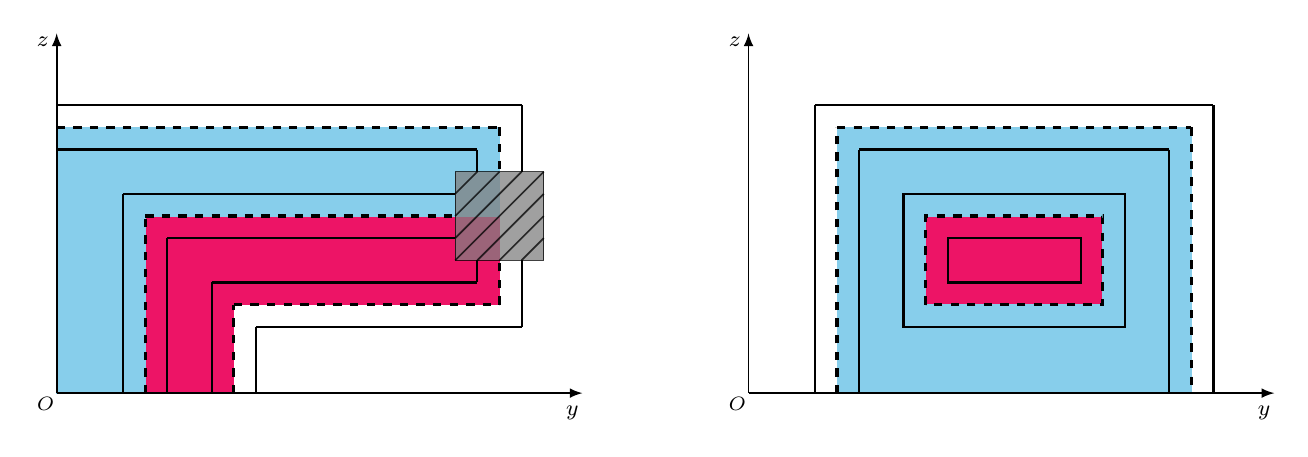
\begin{tikzpicture}[x=0.8cm, y=0.8cm, >=latex, every text node part/.style={align=center}]
    %% BEGIN left picture
    \foreach \x in {1,...,1}
        \foreach \y in {0,...,0} {
            \filldraw [fill=WildStrawberry,draw=WildStrawberry] (32pt*\x,32pt*\y) rectangle (32pt*\x+32pt, 32pt*\y+32pt);
        } 
    \foreach \x in {1,...,4}
        \foreach \y in {1,...,1} {
            \filldraw [fill=WildStrawberry,draw=WildStrawberry] (32pt*\x,32pt*\y) rectangle (32pt*\x+32pt, 32pt*\y+32pt);
        } 
    \foreach \x in {0,...,0}
        \foreach \y in {0,...,1} {
            \filldraw [fill=SkyBlue,draw=SkyBlue] (32pt*\x,32pt*\y) rectangle (32pt*\x+32pt, 32pt*\y+32pt);
        } 
    \foreach \x in {0,...,4}
        \foreach \y in {2,...,2} {
            \filldraw [fill=SkyBlue,draw=SkyBlue] (32pt*\x,32pt*\y) rectangle (32pt*\x+32pt, 32pt*\y+32pt);
        } 

    % \filldraw[draw=Gray,nearly transparent] (144pt, 48pt) rectangle (176pt, 80pt);
    \draw[draw=Black, fill=Gray, nearly opaque] (144pt, 48pt) rectangle (176pt, 80pt);
    \path[semithick,nearly opaque] (144pt,48pt) edge (176pt,80pt);
    \path[semithick,nearly opaque] (144pt,56pt) edge (168pt,80pt);
    \path[semithick,nearly opaque] (144pt,64pt) edge (160pt,80pt);
    \path[semithick,nearly opaque] (144pt,72pt) edge (152pt,80pt);
    \path[semithick,nearly opaque] (152pt,48pt) edge (176pt,72pt);
    \path[semithick,nearly opaque] (160pt,48pt) edge (176pt,64pt);
    \path[semithick,nearly opaque] (168pt,48pt) edge (176pt,56pt);

    \path[Black,very thick,dashed] (32pt, 0pt) edge (32pt, 64pt);
    \path[Black,very thick,dashed] (32pt, 64pt) edge (144pt, 64pt);
    \path[Black,thick] (24pt, 0pt) edge (24pt, 72pt);
    \path[Black,thick] (24pt, 72pt) edge (144pt, 72pt);
    \path[Black,thick] (40pt, 0pt) edge (40pt, 56pt);
    \path[Black,thick] (40pt, 56pt) edge (144pt, 56pt);
    \path[Black,very thick,dashed] (0pt, 96pt) edge (160pt, 96pt);
    \path[Black,very thick,dashed] (160pt, 96pt) edge (160pt, 80pt);
    \path[Black,thick] (0pt, 104pt) edge (168pt, 104pt);
    \path[Black,thick] (168pt, 104pt) edge (168pt, 80pt);
    \path[Black,thick] (0pt, 88pt) edge (152pt, 88pt);
    \path[Black,thick] (152pt, 88pt) edge (152pt, 80pt);
    \path[Black,very thick,dashed] (64pt, 0pt) edge (64pt, 32pt);
    \path[Black,very thick,dashed] (64pt, 32pt) edge (160pt, 32pt);
    \path[Black,very thick,dashed] (160pt, 32pt) edge (160pt, 48pt);
    \path[Black,thick] (56pt, 0pt) edge (56pt, 40pt);
    \path[Black,thick] (56pt, 40pt) edge (152pt, 40pt);
    \path[Black,thick] (152pt, 40pt) edge (152pt, 48pt);
    \path[Black,thick] (72pt, 0pt) edge (72pt, 24pt);
    \path[Black,thick] (72pt, 24pt) edge (168pt, 24pt);
    \path[Black,thick] (168pt, 24pt) edge (168pt, 48pt);

    \path[->,semithick] (0pt, 0pt) edge (0pt, 130pt);
    \path[->,semithick] (0pt, 0pt) edge (190pt, 0pt);
    \node [] () at (-4pt, -4pt) {\scriptsize $O$};
    \node [] () at (186.3pt, -7pt) {\footnotesize $y$};
    \node [] () at (-5pt, 127pt) {\footnotesize $z$};
    %% END left picture

    %% BEGIN left picture
    \foreach \x in {2,...,3}
        \foreach \y in {1,...,1} {
            \filldraw [fill=WildStrawberry,draw=WildStrawberry] (32pt*\x+250pt,32pt*\y) rectangle (32pt*\x+282pt, 32pt*\y+32pt);
        } 
    \foreach \x in {1,...,1}
        \foreach \y in {0,...,2} {
            \filldraw [fill=SkyBlue,draw=SkyBlue] (32pt*\x+250pt,32pt*\y) rectangle (32pt*\x+282pt, 32pt*\y+32pt);
        } 
    \foreach \x in {4,...,4}
        \foreach \y in {0,...,2} {
            \filldraw [fill=SkyBlue,draw=SkyBlue] (32pt*\x+250pt,32pt*\y) rectangle (32pt*\x+282pt, 32pt*\y+32pt);
        } 
    \foreach \x in {2,...,3}
        \foreach \y in {0,...,0} {
            \filldraw [fill=SkyBlue,draw=SkyBlue] (32pt*\x+250pt,32pt*\y) rectangle (32pt*\x+282pt, 32pt*\y+32pt);
        } 
    \foreach \x in {2,...,3}
        \foreach \y in {2,...,2} {
            \filldraw [fill=SkyBlue,draw=SkyBlue] (32pt*\x+250pt,32pt*\y) rectangle (32pt*\x+282pt, 32pt*\y+32pt);
        } 
    
    \draw [draw=Black,very thick,dashed] (314pt, 32pt) rectangle (378pt, 64pt);
    \path [Black,very thick,dashed] (282pt, 0pt) edge (282pt, 96pt);
    \path [Black,very thick,dashed] (282pt, 96pt) edge (410pt, 96pt);
    \path [Black,very thick,dashed] (410pt, 96pt) edge (410pt, 0pt);

    \draw [draw=Black,thick] (306pt, 24pt) rectangle (386pt, 72pt);
    \draw [draw=Black,thick] (322pt, 40pt) rectangle (370pt, 56pt);
    \path [Black,thick] (274pt, 0pt) edge (274pt, 104pt);
    \path [Black,thick] (274pt, 104pt) edge (418pt, 104pt);
    \path [Black,thick] (418pt, 104pt) edge (418pt, 0pt);
    \path [Black,thick] (290pt, 0pt) edge (290pt, 88pt);
    \path [Black,thick] (290pt, 88pt) edge (402pt, 88pt);
    \path [Black,thick] (402pt, 88pt) edge (402pt, 0pt);

    \path[->,semithick] (250pt, 0pt) edge (250pt, 130pt);
    \path[->,semithick] (250pt, 0pt) edge (440pt, 0pt);
    \node [] () at (246pt, -4pt) {\scriptsize $O$};
    \node [] () at (436.3pt, -7pt) {\footnotesize $y$};
    \node [] () at (245pt, 127pt) {\footnotesize $z$};
    %% END left picture
\end{tikzpicture}
    \caption{\small A demonstration of the first steps for our definition of the coordinate converter. 
    Here, we only focus on the region of the coloring that is at most bichromatic because trichromatic regions (e.g., the shadowed part on the left) are \PPAD-hard to find.
    The dashed 1-manifolds represent the ``color switches'' in each instance. 
    We will find the $\ell_{\infty}$ distance (only in terms of the last two coordinates) of each point to these color switches. The solid 1-manifolds represent the sets of points at distance $\eps^2$ to color switches.
    }
    \label{fig:convert}
\end{figure}

\begin{figure}[t]
    \tikzset{%
    every neuron/.style={
        circle,
        draw,
        minimum size=5pt,
        inner sep=0pt,
        very thin
    },
    neuron/.style={
        fill
    },
}

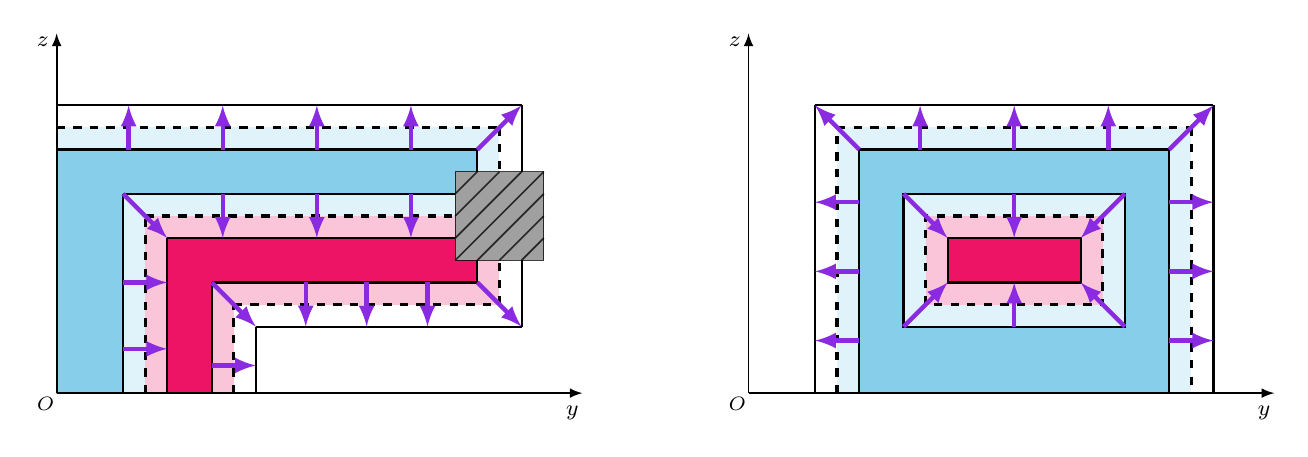
\begin{tikzpicture}[x=0.8cm, y=0.8cm, >=latex, every text node part/.style={align=center}]
    %% BEGIN left picture

    % \filldraw[draw=Gray,nearly transparent] (144pt, 48pt) rectangle (176pt, 80pt);
    \filldraw [fill=SkyBlue,draw=SkyBlue] (0pt,0pt) rectangle (24pt, 88pt);
    \filldraw [fill=SkyBlue,draw=SkyBlue] (24pt,72pt) rectangle (144pt, 88pt);
    \filldraw [fill=SkyBlue,draw=SkyBlue] (144pt,80pt) rectangle (152pt, 88pt);

    \fill[fill=SkyBlue,nearly transparent] (24pt,0pt) rectangle (32pt, 72pt);
    \fill[fill=SkyBlue,nearly transparent] (32pt,64pt) rectangle (144pt, 72pt);
    \fill[fill=SkyBlue,nearly transparent] (0pt,88pt) rectangle (152pt, 96pt);
    \fill[fill=SkyBlue,nearly transparent] (152pt,80pt) rectangle (160pt, 96pt);

    \filldraw [fill=WildStrawberry,draw=WildStrawberry] (40pt,0pt) rectangle (56pt, 56pt);
    \filldraw [fill=WildStrawberry,draw=WildStrawberry] (56pt,40pt) rectangle (144pt, 56pt);
    \filldraw [fill=WildStrawberry,draw=WildStrawberry] (144pt,40pt) rectangle (152pt, 48pt);

    \fill[fill=WildStrawberry,nearly transparent] (32pt,0pt) rectangle (40pt, 64pt);
    \fill[fill=WildStrawberry,nearly transparent] (40pt,56pt) rectangle (144pt, 64pt);
    \fill[fill=WildStrawberry,nearly transparent] (56pt,0pt) rectangle (64pt, 40pt);
    \fill[fill=WildStrawberry,nearly transparent] (64pt,32pt) rectangle (152pt, 40pt);
    \fill[fill=WildStrawberry,nearly transparent] (152pt,32pt) rectangle (160pt, 48pt);

    \draw[draw=Black, fill=Gray, nearly opaque] (144pt, 48pt) rectangle (176pt, 80pt);
    \path[semithick,nearly opaque] (144pt,48pt) edge (176pt,80pt);
    \path[semithick,nearly opaque] (144pt,56pt) edge (168pt,80pt);
    \path[semithick,nearly opaque] (144pt,64pt) edge (160pt,80pt);
    \path[semithick,nearly opaque] (144pt,72pt) edge (152pt,80pt);
    \path[semithick,nearly opaque] (152pt,48pt) edge (176pt,72pt);
    \path[semithick,nearly opaque] (160pt,48pt) edge (176pt,64pt);
    \path[semithick,nearly opaque] (168pt,48pt) edge (176pt,56pt);

    \path[Black,very thick,dashed] (32pt, 0pt) edge (32pt, 64pt);
    \path[Black,very thick,dashed] (32pt, 64pt) edge (144pt, 64pt);
    \path[Black,thick] (24pt, 0pt) edge (24pt, 72pt);
    \path[Black,thick] (24pt, 72pt) edge (144pt, 72pt);
    \path[Black,thick] (40pt, 0pt) edge (40pt, 56pt);
    \path[Black,thick] (40pt, 56pt) edge (144pt, 56pt);
    \path[Black,very thick,dashed] (0pt, 96pt) edge (160pt, 96pt);
    \path[Black,very thick,dashed] (160pt, 96pt) edge (160pt, 80pt);
    \path[Black,thick] (0pt, 104pt) edge (168pt, 104pt);
    \path[Black,thick] (168pt, 104pt) edge (168pt, 80pt);
    \path[Black,thick] (0pt, 88pt) edge (152pt, 88pt);
    \path[Black,thick] (152pt, 88pt) edge (152pt, 80pt);
    \path[Black,very thick,dashed] (64pt, 0pt) edge (64pt, 32pt);
    \path[Black,very thick,dashed] (64pt, 32pt) edge (160pt, 32pt);
    \path[Black,very thick,dashed] (160pt, 32pt) edge (160pt, 48pt);
    \path[Black,thick] (56pt, 0pt) edge (56pt, 40pt);
    \path[Black,thick] (56pt, 40pt) edge (152pt, 40pt);
    \path[Black,thick] (152pt, 40pt) edge (152pt, 48pt);
    \path[Black,thick] (72pt, 0pt) edge (72pt, 24pt);
    \path[Black,thick] (72pt, 24pt) edge (168pt, 24pt);
    \path[Black,thick] (168pt, 24pt) edge (168pt, 48pt);

    \path[->,semithick] (0pt, 0pt) edge (0pt, 130pt);
    \path[->,semithick] (0pt, 0pt) edge (190pt, 0pt);
    \node [] () at (-4pt, -4pt) {\scriptsize $O$};
    \node [] () at (186.3pt, -7pt) {\footnotesize $y$};
    \node [] () at (-5pt, 127pt) {\footnotesize $z$};

    \path[BlueViolet,->,ultra thick] (24pt, 72pt) edge (40pt, 56pt);

    \path[BlueViolet,->,ultra thick] (24pt, 40pt) edge (40pt, 40pt);
    \path[BlueViolet,->,ultra thick] (24pt, 16pt) edge (40pt, 16pt);
    \path[BlueViolet,->,ultra thick] (94pt, 72pt) edge (94pt, 56pt);
    \path[BlueViolet,->,ultra thick] (60pt, 72pt) edge (60pt, 56pt);
    \path[BlueViolet,->,ultra thick] (128pt, 72pt) edge (128pt, 56pt);

    \path[BlueViolet,->,ultra thick] (152pt, 88pt) edge (168pt, 104pt);

    \path[BlueViolet,->,ultra thick] (128pt, 88pt) edge (128pt, 104pt);
    \path[BlueViolet,->,ultra thick] (94pt, 88pt) edge (94pt, 104pt);
    \path[BlueViolet,->,ultra thick] (60pt, 88pt) edge (60pt, 104pt);
    \path[BlueViolet,->,ultra thick] (26pt, 88pt) edge (26pt, 104pt);

    \path[BlueViolet,->,ultra thick] (56pt, 40pt) edge (72pt, 24pt);
    \path[BlueViolet,->,ultra thick] (152pt, 40pt) edge (168pt, 24pt);

    \path[BlueViolet,->,ultra thick] (134pt, 40pt) edge (134pt, 24pt);
    \path[BlueViolet,->,ultra thick] (112pt, 40pt) edge (112pt, 24pt);
    \path[BlueViolet,->,ultra thick] (90pt, 40pt) edge (90pt, 24pt);
    \path[BlueViolet,->,ultra thick] (56pt, 10pt) edge (72pt, 10pt);
    %% END left picture

    %% BEGIN left picture
    \fill[fill=SkyBlue,nearly transparent] (306pt,24pt) rectangle (314pt, 72pt);
    \fill[fill=SkyBlue,nearly transparent] (314pt,24pt) rectangle (386pt, 32pt);
    \fill[fill=SkyBlue,nearly transparent] (314pt,64pt) rectangle (386pt, 72pt);
    \fill[fill=SkyBlue,nearly transparent] (378pt,32pt) rectangle (386pt, 64pt);
    \fill[fill=SkyBlue,nearly transparent] (282pt,0pt) rectangle (290pt, 96pt);
    \fill[fill=SkyBlue,nearly transparent] (402pt,0pt) rectangle (410pt, 96pt);
    \fill[fill=SkyBlue,nearly transparent] (290pt,88pt) rectangle (402pt, 96pt);

    \filldraw [fill=SkyBlue,draw=SkyBlue] (290pt,0pt) rectangle (306pt, 88pt);
    \filldraw [fill=SkyBlue,draw=SkyBlue] (386pt,0pt) rectangle (402pt, 88pt);
    \filldraw [fill=SkyBlue,draw=SkyBlue] (306pt,0pt) rectangle (386pt, 24pt);
    \filldraw [fill=SkyBlue,draw=SkyBlue] (306pt,72pt) rectangle (386pt, 88pt);

    \fill[fill=WildStrawberry,nearly transparent] (314pt,32pt) rectangle (378pt, 64pt);
    \filldraw [fill=WildStrawberry,draw=WildStrawberry] (322pt,40pt) rectangle (370pt, 56pt);

    \draw [draw=Black,very thick,dashed] (314pt, 32pt) rectangle (378pt, 64pt);
    \draw [draw=Black,thick] (306pt, 24pt) rectangle (386pt, 72pt);
    \draw [draw=Black,thick] (322pt, 40pt) rectangle (370pt, 56pt);

    \path [Black,very thick,dashed] (282pt, 0pt) edge (282pt, 96pt);
    \path [Black,very thick,dashed] (282pt, 96pt) edge (410pt, 96pt);
    \path [Black,very thick,dashed] (410pt, 96pt) edge (410pt, 0pt);
    \path [Black,thick] (274pt, 0pt) edge (274pt, 104pt);
    \path [Black,thick] (274pt, 104pt) edge (418pt, 104pt);
    \path [Black,thick] (418pt, 104pt) edge (418pt, 0pt);
    \path [Black,thick] (290pt, 0pt) edge (290pt, 88pt);
    \path [Black,thick] (290pt, 88pt) edge (402pt, 88pt);
    \path [Black,thick] (402pt, 88pt) edge (402pt, 0pt);

    \path[->,semithick] (250pt, 0pt) edge (250pt, 130pt);
    \path[->,semithick] (250pt, 0pt) edge (440pt, 0pt);
    \node [] () at (246pt, -4pt) {\scriptsize $O$};
    \node [] () at (436.3pt, -7pt) {\footnotesize $y$};
    \node [] () at (245pt, 127pt) {\footnotesize $z$};

    \path[BlueViolet,->,ultra thick] (306pt, 24pt) edge (322pt, 40pt);
    \path[BlueViolet,->,ultra thick] (306pt, 72pt) edge (322pt, 56pt);
    \path[BlueViolet,->,ultra thick] (386pt, 24pt) edge (370pt, 40pt);
    \path[BlueViolet,->,ultra thick] (386pt, 72pt) edge (370pt, 56pt);

    \path[BlueViolet,->,ultra thick] (346pt, 24pt) edge (346pt, 40pt);
    % \path[BlueViolet,->,ultra thick] (332pt, 24pt) edge (332pt, 40pt);
    % \path[BlueViolet,->,ultra thick] (360pt, 24pt) edge (360pt, 40pt);
    \path[BlueViolet,->,ultra thick] (346pt, 72pt) edge (346pt, 56pt);

    
    \path[BlueViolet,->,ultra thick] (290pt, 88pt) edge (274pt, 104pt);
    \path[BlueViolet,->,ultra thick] (402pt, 88pt) edge (418pt, 104pt);

    \path[BlueViolet,->,ultra thick] (346pt, 88pt) edge (346pt, 104pt);
    \path[BlueViolet,->,ultra thick] (312pt, 88pt) edge (312pt, 104pt);
    \path[BlueViolet,->,ultra thick] (380pt, 88pt) edge (380pt, 104pt);
    \path[BlueViolet,->,ultra thick] (290pt, 69pt) edge (274pt, 69pt);
    \path[BlueViolet,->,ultra thick] (290pt, 44pt) edge (274pt, 44pt);
    \path[BlueViolet,->,ultra thick] (290pt, 19pt) edge (274pt, 19pt);
    \path[BlueViolet,->,ultra thick] (402pt, 69pt) edge (418pt, 69pt);
    \path[BlueViolet,->,ultra thick] (402pt, 44pt) edge (418pt, 44pt);
    \path[BlueViolet,->,ultra thick] (402pt, 19pt) edge (418pt, 19pt);
    %% END left picture
\end{tikzpicture}
    \caption{\small A demonstration of the second steps for our definition of the coordinate converter. 
    Here, we focus on the region of the coloring that is at most bichromatic.
    Suppose the colors of the blue\,/\,red\,/\,white regions are respectively indexed by 1\,/\,2\,/\,3. 
    For each ``color switch'', we draw arrows from the 1-manifold that is $\eps^2$ away from it and has the lower index to the 1-manifold that is $\eps^2$ away from it and has the higher index.
    The region covered by the arrows are {\em hot regions}.
    Points on the sources of the arrows will have a converted coordinate of $0$, while those on the sinks will have a converted coordinate of $1$.
    We give converted coordinates for other points on the arrows according to their distances to the sources. 
    Points not on any arrow will be marked as either {\em warm} or {\em cold}. 
    }
    \label{fig:convert2}
\end{figure}

\paragraph{Definition.} 
Mathematically, the coordinate converter is defined via the nearest differently colored points. 
More specifically, we consider the $\ell_\infty$ distance on the second and the third coordinate:
\begin{align}
    \label{eqn:modified-distance}
    d(\vec{x}, \vec{y}) := \max\set{|x_2-y_2|, |x_3-y_3|}
\end{align} 
For each point $\vec{x}\in \Delta^2$, we find the infimum distance among all points with a fixed color $c\neq C(\vec{x})$: 
\begin{align}\label{eq:d_min}
    d_{\min}(\vec{x}, c) = \inf_{\vec{y}\in \Delta^2: C(\vec{y})=c} 
    d(\vec{x}, \vec{y})
    ~,
\end{align}
and we define its {\em neighboring color} by 
\begin{align}
    \label{eqn:cnn}
    C_{\sf nn}(\vec{x}) = \argmin_{c\in [3]:c\neq C(\vec{x})} \left(d_{\min}(\vec{x}, c),\ c\right)~.
\end{align}
That is, its neighboring color is defined as the color $c$ that takes the minimum infimum distance $d_{\min}(\vec{x}, c)$, breaking ties by choosing the color with the smallest index.
Or equivalently, the neighboring color of a point equals the different color on the nearest ``color switch'' from the point. 
With this definition of neighboring colors, we define the {\rm nearest neighbor} as the point that attains the minimum in~\cref{eq:d_min}, i.e.:
\begin{align}
    \label{eqn:nn}
    \nn(\vec{x}) = \arginf_{\vec{y}\in \Delta^2: C(\vec{y})=C_{\sf nn}(\vec{x},C)} d(\vec{x}, \vec{y})~.
\end{align}
Note that the color on the nearest neighbor of $\vec{x}$ may be the same as the color on $\vec{x}$, but it must correspond to the limit of an infinite sequence of points that have different colors than $\vec{x}$.
Finally, we define the coordinate converter $\rel$ 
as follows. (The coordinate converter is defined {\em relative to the nearest neighbor}, hence its name.)
We divide the entire $2$-simplex into different regions based on each point's {\em distance to the nearest neighbor}, i.e., $d(\vec{x}, \nn(\vec{x}))$.
\begin{itemize}[itemsep=0.2em,topsep=0.5em]
    \item The {\em hot} region consists of points having distance to the nearest neighbor strictly less than $\eps^2$, i.e., points $\vec{x}$ with $d(\vec{x}, \nn(\vec{x}))<\eps^2$; we say that points in this region are {\em hot}.
    \item The {\em warm} region consists of points having distance to the nearest neighbor between $\eps^2$ (inclusive) and $2\eps^2$ (exclusive), i.e., points $\vec{x}$ with $d(\vec{x}, \nn(\vec{x}))\in [\eps^2,2\eps^2)$; we say that points in this region are {\em warm}.
    \item The {\em cold} region consists of points having distance to the nearest neighbor no less than $2\eps^2$, i.e., points $\vec{x}$ with $d(\vec{x}, \nn(\vec{x}))\geq 2\eps^2$; we say that points in this region are {\em cold}.
\end{itemize}
For points in the {\em hot} region induced by each ``color switch'', 
we map it continuously to a converted coordinate in $(0,1)$, from the boundary with a smaller-indexed color to the boundary with a larger-indexed color.
For points in the {\em warm} region induced by each ``color switch'', we integrally map it to $0$ or $1$ depending on whether its color has a smaller or larger index than that of its neighboring color.
For points in the {\em cold} region, we enforce its converted coordinate to $0$ or $1$ only depending on its own color. 
We summarize the definition in \cref{eqn:coordinate-converter}, where the first two cases are for the {\em hot} and {\em warm} regions and the last two cases are for the {\em cold} region.
\begin{align}
    \label{eqn:coordinate-converter}
    \rel(\vec{x}) = \begin{cases}
        \hfill \left(0.5 - 0.5\eps^{-2} \cdot d(\vec{x}, \vec{nn}(\vec{x}))
        \right)_+ \hfill & \text{if $\vec{x}$ is {\em hot\,/\,warm} and $C_{\sf nn}(\vec{x})>C(\vec{x})$,}\\
        \left(0.5 + 0.5\eps^{-2} \cdot d(\vec{x}, \vec{nn}(\vec{x}))\right)_- & \text{if $\vec{x}$ is {\em hot\,/\,warm} and $C_{\sf nn}(\vec{x})<C(\vec{x})$,}\\
        \hfill 0 \hfill & \text{if $\vec{x}$ is {\em cold} and $C(\vec{x})=1$,}\\
        \hfill 1 \hfill & \text{if $\vec{x}$ is {\em cold} and $C(\vec{x})\in \{2,3\}$.}
    \end{cases}
\end{align}
Because warm points satisfy $d(\vec{x},\nn(\vec{x}))\geq \eps^2$ and hot points are those with $d(\vec{x}, \nn(\vec{x}))<\eps^2$, we have the following fact.
\begin{fact}
    \label{fact:hot-versus-value}
    For any point $\vec{x}\in \Delta^2$, we have $\rel(\vec{x})\in (0,1)$ if and only if $\vec{x}$ is hot.
\end{fact}
As discussed above, our use of this coordinate converter is to convert each point $\vec{x}\in \Delta^3$ to $((1-x_4)\cdot (1-\rel(\vec{P}(\vec{x}))), (1-x_4)\cdot \rel(\vec{P}(\vec{x})), x_4)\in \Delta^2$.
If $\vec{P}(\vec{x})$ is warm or cold, $\rel(\vec{P}(\vec{x}))=0$ and $\vec{x}$ will be converted to either $(1-z,0,z)$ or $(0,1-z,z)$ for $z=x_4$. 
Recall \cref{lem:base-instance-lr-boundaries}, where we have shown for $C$ that
\begin{align*}
 \forall z\in [0,1], \quad \quad & \hfill C(1-z,0,z) = \begin{cases}
    1 & z\leq 0.1~, \\
    3 & z>0.1~;
 \end{cases}
 \hfill
 &
 \hfill
 C(0,1-z,z) = \begin{cases}
    2 & z\leq 0.1~, \\
    3 & z>0.1~.
 \end{cases}
 \hfill
\end{align*} 
One unified way to interpret this coloring is to consider the colors on the line segments $(1-z,0,z)$ and $(0,1-z,z)$ as functions of $z \in [0,1]$: when $z > 0.1$ they take their color from $(0,0,1)$, and when $z \le 0.1$ they take the color of the other endpoint. 
This symmetry will be useful later when we that there is no spurious solutions are created where two warm\,/\,cold points are close to each other but have a different converted coordinate (i.e., one equals $0$, but the other equals $1$). 
Therefore, we can consider the following equivalence between the converted coordinates.

\begin{definition}[Equivalence between converted coordinates]
    \label{def:equiv-converted-coordinates}
    For any converted coordinates $\tilde{x}, \tilde{x}'\in [0,1]$, we say they are equivalent (denoted as $\tilde{x}\simrel \tilde{x}'$) if we have either $\tilde{x}=\tilde{x}'$ or $\tilde{x},\tilde{x}'\in \{0,1\}$. 
\end{definition}

\begin{claim}
    \label{lem:color-equiv-for-converted}
    For any converted coordinates $\tilde{x}, \tilde{x}'\in [0,1]$ such that $\tilde{x}\sim \tilde{x}'$, and any $z\in [0,1]$, we have 
    \begin{align*}
        C((1-z)\cdot (1-\tilde{x}), (1-z)\cdot \tilde{x}, z) = C((1-z)\cdot (1-\tilde{x}'), (1-z)\cdot \tilde{x}', z)~.
    \end{align*}
\end{claim}

\subsubsection{Key properties of the coordinate converter}
Next, we establish the key properties about the coordinate converter on this family of instances.

\paragraph{Property I: Polynomial time computation}
First, we show that all previous functions can be 
``roughly'' 
implemented in polynomial time and we can thus use them freely in our reduction.
That is, we can always output the true converted coordinate $\rel$ and, whenever $\vec{x}$ is hot or warm (i.e., $d(\vec{x}, \nn(\vec{x}))<2\eps^2$), we can also output the neighboring color $C_{\sf nn}(\vec{x})$.

\begin{lemma}
    \label{lem:poly-time-oracle-and-converter}
    Given oracle access to $C$, there is a polynomial-time algorithm that takes any $\vec{x}\in \Delta^2$ as input and that outputs 
    $\rel(\vec{x})$.
    Furthermore, if $d(\vec{x}, \nn(\vec{x}))<2\eps^2$, the algorithm can also compute $C_{\sf nn}(\vec{x})$ in polynomial time.
\end{lemma}
\begin{proof}
    According to our definition of the coordinate converter~\cref{eqn:coordinate-converter}, it suffices to only compute the exact value of $d(\vec{x}, \nn(\vec{x}))$ for $\vec{x}$ such that $d(\vec{x}, \nn(\vec{x}))\leq 2\eps^2$.
    The value of $d(\vec{x}, \nn(\vec{x}))$ can be computed by its distance to each ``color switch''. 
    Note that we only have a constant number of all the color switches outside the core  region  are defined by $O(1)$ line segments (\cref{alg:base-instance}, or see \cref{fig:continuous-mapping}), thus we can enumerate over them. 
    For those ``color switches'' strictly inside the core region, because each point in $C_{\rect}$ is transformed into a $1.6\eps\times 1.6\eps$ square (\cref{alg:base-instance}) and $0.8\eps \gg 2\eps^2$, we only need to check at most $8$ points in the 2{\rm D}-\rect\Sperner instance $C_{\rect}$, which can be done by querying the oracle of $C$ according to \cref{alg:base-instance}.
\end{proof}

\paragraph{Property II: Symmetry}
As mentioned earlier, we will use the converted coordinate with a new coordinate (in a higher dimension) to embed a new copy of the 2{\rm D}-\Sperner instance inside our construction.
That is, supposing the converted coordinate is $\tilde{x}$ and the new coordinate is $z$, we will define a vector, $((1-z)\cdot (1-\tilde{x}), (1-z)\cdot \tilde{x}, z)$, 
for the new copy. 
Later, to argue that there is no issue arising from the fact that we can have very close points with a converted coordinate of $\tilde{x}=0$ and of $\tilde{x}=1$, we also need the following property that the converted coordinates of $(1-z,0,z)$ and $(0,1-z,z)$ are equivalent and their neighboring colors are symmetric. 
This stronger symmetry also implies a characterization of the temperature on the boudnary:
\begin{itemize}[itemsep=0.2em,topsep=0.5em]
    \item If $z\in 0.1\pm \eps^2$, points $(1-z,0,z)$ and $(0,1-z,z)$ are {\em hot} and the converted coordinate equals $0.5+0.5\eps^{-2}\cdot(z-0.1)$.
    \item If $z\in 0.1\pm 2\eps^2$ but $z\notin 0.1\pm \eps^2$, points $(1-z,0,z)$ and $(0,1-z,z)$ are {\em warm} and the converted coordinate is the rounding of $0.5+0.5\eps^{-2}\cdot(z-0.1)$ to its nearest integer in $\{0,1\}$.
    \item If $z\notin 0.1\pm 2\eps^2$, points $(1-z,0,z)$ and $(0,1-z,z)$ are {\em cold} and the converted coordinate is in $\{0,1\}$ (where we don't care its exact value).
\end{itemize}
Here, the value of $|z-0.1|$ gives the {\em hot} and {\em warm} points' distances to their nearest neighbor. 

\begin{lemma}[Symmetry on converted coordinate]
    \label{lem:symmetry-on-converted-coordinates}
    Warm and hot points on the line segments $(1-x_3, 0,x_3)$ and $(0, 1-x_3,x_3)$ have $x_3\in 0.1\pm 2\eps^2$. For any such $x_3$, we have 
    \begin{align}
        \label{eqn:stronger-symmetry-on-converted-coordinates}
        \rel(1-x_3, 0,x_3) = \left(1/2 + \frac{x_3-0.1}{2 \eps^2}\right)_{[0,1]} =\rel(0, 1-x_3, x_3)~,
    \end{align}
    and the neighboring color is characterized as follows
    \begin{align*}
        C_{\sf nn}(1-x_3,0,x_3) = \begin{cases}
            3 & \text{if $x_3\leq 0.1$,}\\
            1 & \text{if $x_3>0.1$,}
        \end{cases}
        \quad
        \text{and}
        \quad
        C_{\sf nn}(0,1-x_3,x_3) = \begin{cases}
            3 & \text{if $x_3\leq 0.1$,}\\
            2 & \text{if $x_3>0.1$.}
        \end{cases}
    \end{align*}
\end{lemma}
\begin{proof}
    Note that we guarantee our coloring to satisfy all the following equations.
    \begin{align*}
        \forall \vec{y}\in \Delta^2, \quad
        \begin{cases}
        C(\vec{y}) = 1 & \quad \text{if } y_3\leq 0.1, y_2\leq  0.5~,\\
        C(\vec{y}) = 2 & \quad \text{if } y_3\leq 0.1, y_2> 0.5~,\\
        C(\vec{y}) = 3 & \quad \text{if } y_3> 0.1, y_2\notin 0.5\pm 0.1~,\\
        C(\vec{y}) = 3 & \quad \text{if } y_3>0.3 ~.\\
        \end{cases}
    \end{align*}

    \paragraph{Consider any $x_3\leq 0.1$.} 
    We have $C(1-x_3,0,x_3)=1$ and $C(0,1-x_3,x_3)=2$. 
    Note that any point $\vec{y}$ that has color other than $1$ has either $y_3\geq 0.1$ or $y_2>0.5$. 
    Hence, we have $\vec{nn}(1-x_3,0,x_3)=(0.9,0,0.1)$ for any $x_3\leq 0.1$. 
    We then have $d((1-x_3,0,x_3), \vec{nn}(1-x_3,0,x_3))=0.1-x_3$ and $C_{\sf nn}(1-x_3,0,x_3)=3$.
    According to the definition of the coordinate converter \cref{eqn:coordinate-converter}, if $0.1-x_3< 2\eps^2$ (i.e., $x_3> 0.1-2\eps^2$), the point $(1-x_3,0,x_3)$ is hot or warm, and
    \begin{align*}
        \rel(1-x_3,0,x_3) = \left(0.5-0.5\eps^{-2}\cdot (0.1-x_3)\right)_+ = \left(0.5 + \frac{x_3-0.1}{2\eps^2}\right)_{[0,1]}~,
    \end{align*}
    which matches \cref{eqn:stronger-symmetry-on-converted-coordinates}.
    Otherwise, we have $d((1-x_3,0,x_3), \vec{nn}(1-x_3,0,x_3))\geq 2\eps^2$ and thus the point $(1-x_3,0,x_3)$ is cold.
    Similarly, for any $x_3\leq 0.1$, we have $\vec{nn}(0,1-x_3,x_3)=(0,0.9,0.1)$, $d((0,1-x_3,x_3), \vec{nn}(0,1-x_3,x_3))=0.1-x_3$, and $C_{\sf nn}(0,1-x_3,x_3)=3$.
    According to the definition of the temperature, if $x_3>0.1-2\eps^2$, the point $(0,1-x_3,x_3)$ is hot or warm, and we can obtain the right-handed-side equation of \cref{eqn:stronger-symmetry-on-converted-coordinates} according to \cref{eqn:coordinate-converter}. 
    Otherwise, we have $d((0,1-x_3,x_3), \vec{nn}(0,1-x_3,x_3))\geq 2\eps^2$, which implies that the point $(0,1-x_3,x_3)$ is cold.

    \paragraph{Consider any $x_3>0.1$.}
    We have $C(1-x_3,0,x_3)=C(0,1-x_3,x_3)=3$. 
    Note that any point $\vec{y}$ that has color other than $3$ has either $y_3\leq 0.1$ or $y_2\in [0.4, 0.6]$.
    Hence, if $x_3\geq 0.1+2\eps^2$, we have $d((1-x_3,0,x_3), \nn(1-x_3,0,x_3))\geq 2\eps^2$ and thus the point $(1-x_3,0,x_3)$ is cold.
    Otherwise, if $x_3<0.1+2\eps^2$, we have $\nn(1-x_3,0,x_3)=(0.9,0,0.1)$. 
    We then have $d((1-x_3,0,x_3), \vec{nn}(1-x_3,0,x_3))=z-0.1<2\eps^2$ and $C_{\sf nn}(1-x_3,0,x_3)=1$.
    The point $(1-x_3,0,x_3)$ is hot or warm in this case. 
    Further, according to the definition of the coordinate converter \cref{eqn:coordinate-converter}, 
    \begin{align*}
        \rel(1-x_3,0,x_3) = \left(0.5+0.5\eps^{-2}\cdot (x_3-0.1)\right)_- = \left(0.5+ \frac{x_3-0.1}{2\eps^{2}} \right)_{[0,1]},
    \end{align*}
    matching \cref{eqn:stronger-symmetry-on-converted-coordinates}.
    On the other hand, note that any point $\vec{y}$ has color other than $3$ and $y_3\geq 0.1$ must have $y_2+y_3\leq 0.9$. 
    The distance $d$ between $(0,1-x_3,x_3)$ and any such point is at least $0.05$.
    Note that $0.05\gg 2\eps^2$.
    Hence, when $x_3\geq 0.1+2\eps^2$, we have $d((0,1-x_3,x_3), \nn(0,1-x_3,x_3))\geq 2\eps^2$ and thus according to 
    the definition of the temperature, 
    the point $(0,1-x_3,x_3)$ is cold. 
    Otherwise, if $x_3<0.1+2\eps^2$, we have $\nn(0,1-x_3,x_3) = (x_3-0.1,1-x_3,0.1)$. 
    We then have $d((0,1-x_3,x_3), \vec{nn}(0,1-x_3,x_3))=x_3-0.1$ and $C_{\sf nn}(0,1-x_3,x_3)=2$.
    According to the definition of the coordinate converter \cref{eqn:coordinate-converter}, 
    \begin{align*}
        \rel(0,1-x_3,x_3) = \left(0.5+0.5\eps^{-2}\cdot(x_3-0.1)\right)_-  = \left(0.5+ \frac{x_3-0.1}{2\eps^2}\right)_{[0,1]},
    \end{align*}
    matching \cref{eqn:stronger-symmetry-on-converted-coordinates}.
\end{proof}

\begin{corollary}
    \label{lem:converted-equiv-for-converted}
    For any converted coordinates $\tilde{x}, \tilde{x}'\in [0,1]$ such that $\tilde{x}\sim \tilde{x}'$, and any $z\in [0,1]$, we have 
    \begin{align*}
        \rel((1-z)\cdot (1-\tilde{x}), (1-z)\cdot \tilde{x}, z) \,\simrel\, \rel((1-z)\cdot (1-\tilde{x}'), (1-z)\cdot \tilde{x}', z)~.
    \end{align*}
\end{corollary}

\paragraph{Property III: Lipshitzness}  
We show that the coordinate converter is Lipschitz in bichromatic regions in the following sense: consider we view the interval $[0,1]$ as a loop, where $0,1$ corresponds to the same point on the loop, and the distance between any $\rel(\vec{x})$ and $\rel(\vec{x'})$ on the loop can be upper bounded by a $\poly(1/\eps)$ factor of the distance between $\vec{x}$ and $\vec{x'}$. 
We say a point is in a bichromatic region if its neighbourhood, defined in \cref{def:neighbourhood}, is bichromatic.
And, the Lipschitzness property is formalized by \cref{lem:lipschitz-of-the-converter} with a slightly stronger argument.

\begin{definition}
    \label{def:neighbourhood}
    Let $\eps=2^{-n}$.
    For any $\vec{x} \in \Delta^{2}$, let $\mathcal{N}(\vec{x})=\settxt{\vec{y}\in \Delta^2: |x_2-y_2|, |x_3-y_3|\leq \eps/2}$ denote the neighbourhood of $\vec{x}$ with a side length of $\eps$. 
\end{definition}

\begin{lemma}
    \label{lem:lipschitz-of-the-converter}
    For any coloring $C$ and any pair of points $\vec{x}, \vec{x'}$, at least one of the following properties is satisfied:
    \begin{itemize}[itemsep=0em]
        \item {\bf one is in a trichromatic region:} there are three different colors in $\mathcal{N}(\vec{x})$ (or, $\mathcal{N}(\vec{x'})$);
        \item {\bf Lipschitz in the hot\&warm regions:} $|\rel(\vec{x})-\rel(\vec{x'})|\leq \eps^{-2}\cdot \normtxt{\vec{x}-\vec{x'}}{\infty}$; 
        \item {\bf both are in the warm\&cold regions:} $\rel(\vec{x}),\rel(\vec{x'})\in \{0,1\}$. 
    \end{itemize}
\end{lemma}
\begin{proof}
    It suffices to show that the Lipschitz property, $|\rel(\vec{x})-\rel(\vec{x'})|\leq \eps^{-2} \cdot \normtxt{\vec{x}-\vec{x'}}{\infty}$, under the following three assumptions: (1) $\mathcal{N}(\vec{x})$ and $\mathcal{N}(\vec{x'})$ are both at most bichromatic; (2) $\normtxt{\vec{x}-\vec{x'}}{\infty} < \eps^2$; and (3) $\rel(\vec{x})\in (0,1)$ (equivalently by \cref{fact:hot-versus-value}, $d(\vec{x}, \nn(\vec{x}))<\eps^2$). 
    The second assumption makes sense because $\rel(\vec{x}), \rel(\vec{x'})\in [0,1]$ and the second property can trivially hold if the assumption is violated.
    In addition, the second and the third assumption ensures that $d(\vec{x}, \nn(\vec{x})), d(\vec{x'}, \nn(\vec{x'})) < 2\eps^2$, which
    can be obtained by the triangle inequality when $\vec{x}, \vec{x'}$ have the same color and otherwise is trivial by the second assumption.
    This ensures that we must go to the first two cases of \cref{eqn:coordinate-converter} when computing the converted coordinates of $\vec{x}, \vec{x'}$. 
    Next, we discuss two cases on the colors of $\vec{x}$ and $\vec{x'}$.

    \paragraph{Case 1: $\vec{x}$ and $\vec{x'}$ have different colors.}
    Since $d(\vec{x},\vec{x'})\leq \normtxt{\vec{x}-\vec{x'}}{\infty}$, we have 
    $d(\vec{x}, \vec{nn}(\vec{x}))\leq \normtxt{\vec{x}-\vec{x'}}{\infty}$ and $d(\vec{x'}, \vec{nn}(\vec{x'}))\leq \normtxt{\vec{x}-\vec{x'}}{\infty}$.
    According to \cref{eqn:coordinate-converter}, we have
    \begin{align*}
        \rel(\vec{x}) &\in 0.5 \pm 0.5\eps^{-2} \cdot d(\vec{x}, \vec{nn}(\vec{x})) \subseteq 0.5 \pm 0.5\eps^{-2} \cdot \norm{\vec{x}-\vec{x'}}{\infty}~, \quad \text{and}\\
        \rel(\vec{x'}) &\in 0.5 \pm 0.5\eps^{-2} \cdot d(\vec{x'}, \vec{nn}(\vec{x'})) \subseteq 0.5 \pm 0.5\eps^{-2} \cdot \norm{\vec{x}-\vec{x'}}{\infty}~.
    \end{align*}
    Therefore, we have $\abstxt{\rel(\vec{x})-\rel(\vec{x'})}\leq \eps^{-2} \cdot \normtxt{\vec{x}-\vec{x'}}{\infty}$.

    \paragraph{Case 2: $\vec{x}$ and $\vec{x'}$ have the same color.}
    Suppose that $c:=C(\vec{x})=C(\vec{x'})$.
    Because of the definition of the coordinate converter (\cref{eqn:coordinate-converter}), the third assumption implies $d(\vec{x}, \vec{nn}(\vec{x}))<\eps^2$.
    Since $C(\vec{x})\neq C_{\sf nn}(\vec{x})$, according to the definition of the neighbourhood $\mathcal{N}(\vec{x})$ (\cref{def:neighbourhood}), this further implies that $\mathcal{N}(\vec{x})$ is bichromatic combined with our first assumption.
    Suppose that $c'$ is the other color in $\mathcal{N}(\vec{x})$. 
    Or say, $c':=C_{\sf nn}(\vec{x})$. 
    Recall that we have showed that $d(\vec{x'}, \nn(\vec{x'}))<2\eps^{2}$.
    Note that the following set is strictly contained in $\mathcal{N}(\vec{x})$:
    \begin{align*}
        \set{\vec{y}\in \Delta^2: y_2\in x'_2\pm 2\eps^2, y_3\in x'_3\pm 2\eps^2}~.
    \end{align*}
    We don't have any color other than $c,c'$ within a distance of $\eps^2$ from $\vec{x'}$, and thus $C_{\sf nn}(\vec{x'}) =  c'$.
    This means 
    \begin{align*}
        d(\vec{x}, \vec{nn}(\vec{x})) &= d_{\min}(\vec{x}, c') = \inf_{\vec{y}\in \Delta^2: C(\vec{y})=c'} d(\vec{x}, \vec{y})~,\\
        d(\vec{x'}, \vec{nn}(\vec{x'})) &= d_{\min}(\vec{x'}, c') = \inf_{\vec{y}\in \Delta^2: C(\vec{y})=c'} d(\vec{x'}, \vec{y})~.
    \end{align*}
    Therefore, we have
    \begin{align*}
        \abs{d(\vec{x}, \vec{nn}(\vec{x}))-d(\vec{x'}, \vec{nn}(\vec{x'}))} &= \abs{\inf_{\vec{y}\in \Delta^2: C(\vec{y})=c'} d(\vec{x}, \vec{y}) - \inf_{\vec{y}\in \Delta^2: C(\vec{y})=c'} d(\vec{x'}, \vec{y})}
        \\
        &\leq \inf_{\vec{y}\in \Delta^2: C(\vec{y})=c'} \abs{d(\vec{x}, \vec{y})-d(\vec{x'},\vec{y})}
        \\
        &\leq 2\norm{\vec{x}-\vec{x'}}{\infty}~.
    \end{align*}
    Because $C(\vec{x})=c=C(\vec{x'})$ and $C_{\sf nn}(\vec{x}) = c' = C_{\sf nn}(\vec{x'})$, when we compute $\rel(\vec{x})$ and $\rel(\vec{x'})$, we follow the same case of \cref{eqn:coordinate-converter}. 
    Hence, 
    \begin{align*}
        \abs{\rel(\vec{x}) - \rel(\vec{x'})} \leq 0.5\eps^{-2} \cdot \abs{d(\vec{x}, \vec{nn}(\vec{x}))-d(\vec{x'}, \vec{nn}(\vec{x'}))} \leq \eps^{-2} \cdot \norm{\vec{x}-\vec{x'}}{\infty}~,
    \end{align*}
    and we have obtained the lemma for this case.
\end{proof}

Furthermore, a very similar (and slightly simpler) Lipschitzness can be established for points on the two boundaries other than the base $1$-simplex. 
The proof is much simpler -- we only need to do simple calculations based on our previous characterization of the coordinate converter (\cref{lem:symmetry-on-converted-coordinates}).
The technical proof is deferred to \cref{proof:lipschitz-of-the-converter-on-boundaries}.
\begin{restatable}[]{lemma}{repii}
    \label{lem:lipschitz-of-the-converter-on-boundaries}
    For any $z,z'\in [0,1]$ and any pair of points $\vec{x}, \vec{x'}$ such that $\vec{x}\in \{(0,1-z,z),\, (1-z,0,z)\}$ and $\vec{x'}\in \{(0,1-z',z'),\, (1-z',0,z')\}$, at least one of the following properties is satisfied:
    \begin{itemize}[itemsep=0em]
        \item {\bf Lipschitz in the hot\&warm regions:} $|\rel(\vec{x})-\rel(\vec{x'})|\leq \eps^{-2}\cdot |z-z'|$; 
        \item {\bf both are in the warm\&cold regions:} $\rel(\vec{x}),\rel(\vec{x'})\in \{0,1\}$. 
    \end{itemize}
\end{restatable}

\paragraph{Property IV: Cold on the top}
Finally, we show that the points that have reasonably high values on the third dimension ($x_3>0.5$) are all cold. 
This lemma will help ensure that there are no spurious solutions in which any of the three points has a coordinate that has a very high value (e.g., $>1-2^{-\Omega(n)}$) in any of its $\ell$-th projection step (see \cref{def:lth-projection} and next subsection for details). 

\begin{fact}
    \label{lem:trivial-converter}
    For any $\vec{x}\in \Delta^{2}$ such that $x_3\geq 0.5$, we have $\rel(\vec{x})=1$.
\end{fact}
\begin{proof}
    According to \cref{alg:base-instance}, we have $C(\vec{x})=3$ for any $\vec{x}\in \Delta^2$ such that $x_3>0.3$. 
    Therefore, if $x_3\geq 0.5$, $d(\vec{x}, \vec{nn}(\vec{x}))\geq 0.2\gg 2\eps^2$ and thus $\vec{x}$ is cold. 
    According to \cref{eqn:coordinate-converter}, $\rel(\vec{x})=1$. 
\end{proof}

\subsection{Hard instances with three or more dimensions}
\label{subsec:warmup-kd}
In this subsection, we give the constructions for $C^{(k)}$ with $k\geq 3$.
Before giving the construction, for convenience, we introduce the $\ell$-th projection steps we will recursively use to project a point.

\begin{definition}[$\ell$-th projection steps]
    \label{def:lth-projection}
    For any $0\leq \ell\leq k-1$, we use $\vec{P}^{(\ell)}(\vec{x})\in \Delta^{k-\ell}$ to denote the vector we obtain after applying a total number of $\ell$ projection steps on $\vec{x}$, i.e., we let $P^{(0)}(\vec{x})=\vec{x}$ and let $\vec{P}^{(\ell)}(\vec{x}) = \vec{P}(\vec{P}^{(\ell-1)}(\vec{x}))$ for any $ \ell\geq 1$.
\end{definition}

We also define a {\em modified neighbor color} that is consistent with our definition of the coordinate converter for those cold points $\vec{x}$ having $d(\vec{x}, \vec{nn}(\vec{x}))\geq 2\eps^2$.
\begin{align}
    \label{eqn:modified-neighboring-color}
    \hat{C}_{\sf nn}(\vec{x}) = \begin{cases}
        C_{\sf nn}(\vec{x}) & \text{if $d(\vec{x}, \vec{nn}(\vec{x}))< 2\eps^2$,}\\
        \hfill 2 \hfill & \text{if $d(\vec{x}, \vec{nn}(\vec{x})) \geq 2\eps^2$ and $C(\vec{x})=1$,}\\
        \hfill 1 \hfill & \text{if $d(\vec{x}, \vec{nn}(\vec{x})) \geq 2\eps^2$ and $C(\vec{x})\in \{2,3\}$.}
    \end{cases}
\end{align}
The efficient computation of this function follows from \cref{lem:poly-time-oracle-and-converter}.
This will be an auxillary function for our algorithm, which allows us to use the following fact.
\begin{fact}
\label{fact:modified-neighboring-color}
    For any $\vec{x}\in \Delta^2$, we have $C(\vec{x})<\hat{C}_{\sf nn}(\vec{x})$ if $\rel(\vec{x})=0$, and $C(\vec{x})>\hat{C}_{\sf nn}(\vec{x})$ if $\rel(\vec{x})=1$.
\end{fact}

Our construction (formalized in \cref{alg:approx-sperner-kgeq3}) for three or more dimensions is recursive, i.e., we lift $C^{(k)}$ from $C^{(k-1)}$ by the base instance $C$. 
During this process, we recursively compute a sequence of points $\vec{y}^{(2)}, \dots, \vec{y}^{(k)}\in \Delta^2$,  that can each be thought of as a different projection of $\vec{x}$ to a $2$-simplex; additionally, we compute for each $i\in \{2,\dots,k\}$ a palette of three candidate colors $\vec{c}^{(i)}\in \binom{[i+1]}{3}$ that can be used to color the $i$-th copy of $C$; 
in particular, we can use $c^{(k)}_j$ for $j=C(\vec{y}^{(k)})$ as our output color.

In more detail,
our construction begins with projecting $\vec{x}$ to the base $2$-simplex (i.e., letting $\vec{y}^{(2)}=\vec{P}^{(k-2)}(\vec{x})$) and a vector of the only three colors $\vec{c}^{(2)}=(1,2,3)$. 
This initialization is consistent with our $2$-dimensional instance $C^{(2)}$ and the base instance $C$ constructed in \cref{subsec:warmup-2d}.
Then, we recursively lift the $(i-1)$-dimensional instance to the $i$-dimensional instance for each $i\in \{3,\cdots, k\}$ by the following steps:
\begin{enumerate}[itemsep=0.2em, topsep=0.5em]
    \item We locally project the previous projection $\vec{y}^{(i-1)}$ to a point $(1-\tilde{y},\tilde{y})$ on $1$-simplex, using our converted coordinate $\tilde{y}=\rel(\vec{y}^{(i-1)})$. 
    \item We let the new coordinate $z$ (i.e., the next coordinate in $C^{(i)}$) be the last coordinate of $\vec{x}$'s projection to the base $i$-simplex (i.e., $\vec{P}^{(k-i)}(\vec{x})$). 
    Note that this coordinate $z$ was not used in the construction of $C^{(i-1)}$.
    \item With $\tilde{y}$ and $z$, we define our new projection of $\vec{x}$ to a $2$-simplex by $\vec{y}^{(i)}=((1-z)\cdot (1-\tilde{y}), (1-z)\cdot \tilde{y}, z)$, which can be viewed as an weighted average of our previous converted point $(1-\tilde{y}, \tilde{y}, 0)$ on the base $1$-simplex and topmost point $(0,0,1)$ via the new coordinate $z$.
    \item To define the $i$-th palette of three new candidate colors, we look at the previous color $c^{(i-1)}_j$ for $j=C(\vec{y}^{(i-1)})$ and the previous neighboring color $c^{(i-1)}_{j'}$ for $j'=C_{\sf nn}(\vec{y}^{(i-1)})$, and use $c^{(i-1)}_{j}, c^{(i-1)}_{j'}$ and the new color $i+1$ as the three candidate colors. 
\end{enumerate}


\begin{algorithm2e}[t]
    \caption{\outofk Approximate \Sperner Instance $C^{(k)}(\vec{x})$}
    \label{alg:approx-sperner-kgeq3}

    \DontPrintSemicolon
    \SetKwInOut{Input}{Input\,}
    \SetKwInOut{Output}{Output\,}

    \Input{~vector $\vec{x}\in \Delta^k$}

    \Output{~color $c\in [k+1]$}

    $\vec{y}^{(2)} \gets \vec{P}^{(k-2)}(\vec{x})$ \tcp*{initiate $\vec{y}$ by $\vec{x}$'s projection to the base $2$-simplex}

    $\vec{c}^{(2)}\gets (1,2,3)$ \tcp*{initiate the set of 3 colors}

    \For{$i\in \{3,\dots, k\}$}{

        $y_3^{(i)} \gets P_{i+1}^{(k-i)}(\vec{x})$
        \tcp*{find the new $z$-coordinate from the projection of $\vec{x}$}
        \label{line:y_3}

        $y_2^{(i)} \gets (1-y_3^{(i)}) \cdot \rel ( \vec{y}^{(i-1)} )$
        \label{line:y_2}

        $y_1^{(i)} \gets (1-y_3^{(i)})\cdot \left(1-\rel ( \vec{y}^{(i-1)} )\right) $ 
        \tcp*{convert $\vec{y}$ to a point on the $2$-simplex}
        \label{line:y_1}

        $j_1\gets \min \left\{C(\vec{y}^{(i-1)}),\ \hat{C}_{\sf nn}(\vec{y}^{(i-1)})\right\}$

        $j_2\gets \max \left\{C(\vec{y}^{(i-1)}),\ \hat{C}_{\sf nn}(\vec{y}^{(i-1)})\right\}$

        $\vec{c}^{(i)} \gets \left(c_{j_1}^{(i-1)}, c_{j_2}^{(i-1)}, i+1\right)$
        \label{line:obtain-new-set-of-colors}
        \tcp*{obtain the new set of 3 colors}
    }

    $j \gets C \left(\vec{y}^{(k)}\right)$
            
    \Return{$c_j^{(k)}$}
\end{algorithm2e}

Because \cref{alg:approx-sperner-kgeq3} is clearly polynomial-time, in the rest of this subsection, we will prove that we can recover a solution of the $2${\rm D}-\Sperner instance $C$ in polynomial time from any solution of our instances $C^{(k)}$ to finish the analysis. 

\subsubsection{Recovering a 2D solution} 
\label{subsubsec:recovery}

From now on, we assume that the tuple $(\vec{x}^{(1)}, \vec{x}^{(2)}, \vec{x}^{(3)})$ is any good solution for the \outofk Approximate \Sperner instance $C^{(k)}$ satisfying that $\normtxt{\vec{x}^{(i)}-\vec{x}^{(j)}}{\infty}\leq 2^{-3kn}=\eps^3$ for any $i,j\in [3]$. 
We will prove that we can recover a $2${\rm D}-\Sperner solution from it in polynomial time.
\begin{lemma}
    \label{lem:poly-time-recovery}
    Given oracle access to a $2${\rm D}-\Sperner instance $C$ and a tuple of points $(\vec{x}^{(1)}, \vec{x}^{(2)}, \vec{x}^{(3)})$ which satisfy $\normtxt{\vec{x}^{(i)}-\vec{x}^{(j)}}{\infty}\leq 2^{-3kn}$ for any $i,j\in [3]$, and which are trichromatic in the \outofk Approximate \Sperner instance $C^{(k)}$ constructed by \cref{alg:approx-sperner-kgeq3},
    then there is a polynomial-time algorithm that finds a tuple of points $(\vec{\hat{x}}^{(1)}, \vec{\hat{x}}^{(2)}, \vec{\hat{x}}^{(3)})$ which satsify $\normtxt{\vec{\hat{x}}^{(i)}-\vec{\hat{x}}^{(j)}}{\infty}\leq 2^{-n}$ for any $i,j\in [3]$ and which are trichromatic in the $2${\rm D}-\Sperner instance $C$.
\end{lemma}


In the analysis, 
we use $\vec{y}^{(i)}(\vec{x}) = (y^{(i)}_1(\vec{x}), y^{(i)}_2(\vec{x}), y^{(i)}_3(\vec{x}))$
to denote the {\em intermediate projections} we use in \cref{alg:approx-sperner-kgeq3} when the inputs are $\vec{x}$ and $C$. 
Similarly, we use
$\vec{c}^{(i)}(\vec{x}) = (c^{(i)}_1(\vec{x}), c^{(i)}_2(\vec{x}), c^{(i)}_3(\vec{x}))$ 
to denote the {\em intermediate palettes} we use in \cref{alg:approx-sperner-kgeq3} for $\vec{x}$.
In the rest of this section, because the subscripts we will use for $\vec{c}^{(i)}$ can be very complicated, we will use $c_j^{(i)}(\vec{x})$ and $c^{(i)}(\vec{x}, j)$ interchangeably for better presentation.
For any vector $\vec{y}\in \Delta^2$, we use $i^*(\vec{y})$ to denote the first non-zero index of $\vec{y}$, i.e., 
\begin{align}
    \label{eqn:first-nonzero-index}
    i^*(\vec{y}) = \begin{cases}
        1 & \text{if $y_1>0$,}\\
        2 & \text{if $y_1=0$ and $y_2>0$,}\\
        3 & \text{otherwise.}
    \end{cases}
\end{align}


\begin{algorithm2e}[t]
    \caption{Recover a $2${\rm D}-\Sperner solution from \outofk Approximate \Sperner solutions}
    \label{alg:recover-2d-sol}

    \DontPrintSemicolon
    \SetKwInOut{Input}{Input\,}
    \SetKwInOut{Output}{Output\,}

    \Input{~vectors $\vec{x}^{(1)}, \vec{x}^{(2)}, \vec{x}^{(3)}\in \Delta^k$}

    \Output{~vectors $\vec{\hat{x}}^{(1)}, \vec{\hat{x}}^{(2)}, \vec{\hat{x}}^{(3)}\in \Delta^2$}

    \For{$i\in \{2,3,\dots,k-1\}$}{
        \For{$j\in [3]$}{

            \If{$C$ has $3$ different colors in $\mathcal{N}(\vec{y}^{(i)}(\vec{x}^{(j)}))$}{
                $\vec{\hat{x}}^{(1)}, \vec{\hat{x}}^{(2)}, \vec{\hat{x}}^{(3)} \gets $ any 3 points colored differently by $C$ in $\mathcal{N}(\vec{y}^{(i)}(\vec{x}^{(j)}))$\tcp*{the definition of $\vec{y}^{(i)}(\vec{x}^{(j)})$ follows \cref{alg:approx-sperner-kgeq3}}

                \Return{$\vec{\hat{x}}^{(1)}, \vec{\hat{x}}^{(2)}, \vec{\hat{x}}^{(3)}$} \tcp*{trichromatic triangle found while simulation}
            }
        }

    }

    \Return{$\vec{y}^{(k)}(\vec{x}^{(1)}), \vec{y}^{(k)}(\vec{x}^{(2)}), \vec{y}^{(k)}(\vec{x}^{(3)})$}
    \tcp*{trichromatic triangle found when lifting $C^{(k-1)}$ to $C^{(k)}$}
\end{algorithm2e}

Our recovery algorithm (formalized in \cref{alg:recover-2d-sol}) simulates \cref{alg:approx-sperner-kgeq3} for each $\vec{x}^{(j)}$.
At time $i\in [2,k-1]$ when we have computed $\vec{y}^{(i)}(\vec{x}^{(j)})$ for each $j\in [3]$, we examine whether one of them is inside a trichromatic region, i.e., whether $C$ has three different colors in $\mathcal{N}(\vec{y}^{(i)}(\vec{x}^{(j)}))$ for some $j\in [3]$.
Because we turn each point in the 2D-\rect\Sperner instance to a $1.6\eps\times 1.6\eps$ square in the core region, and outside the core region all color switches are defined by $O(1)$ line segments, we can compute all the connected parts of each color within any $\mathcal{N}(\vec{y})$ in polynomial time. 
After we finish the simulation, we simply output $\vec{y}^{(k)}(\vec{x}^{(1)}), \vec{y}^{(k)}(\vec{x}^{(2)}), \vec{y}^{(k)}(\vec{x}^{(3)})$ as a solution for $C$. 

It is clear that any output during the simulation phase of this recovery algorithm gives a valid solution for the 2{\rm D}-\Sperner instance $C$. 
To prove \cref{lem:poly-time-recovery}, we only need to show that the three intermediate projections after the simulation form a valid solution for $C$ if we output after the simulation phase. 
Or equivalently, if each $\vec{y}^{(i)}(\vec{x}^{(j)})$ does not lie in a trichromatic region, the final converted coordinates, $\vec{y}^{(k)}(\vec{x}^{(1)}), \vec{y}^{(k)}(\vec{x}^{(2)}), \vec{y}^{(k)}(\vec{x}^{(3)})$, give a solution for $C$.

Our proof will be considers two cases; the first is where
the given solution $\vec{x}^{(1)}, \vec{x}^{(2)}, \vec{x}^{(3)}$  for $C^{(k)}$ further enjoys the following property: 
\begin{align}
\label{eqn:assumption-for-simple-proof-of-recovery}
\forall 2\leq i\leq k, \forall j\in [3], \quad P_{i+1}^{(k-i)}(\vec{x}^{(j)})\leq 0.9~.
\end{align}
One benefit of first considering this case is that we don't have too crazy projections in \cref{alg:recover-2d-sol}, which can help us significantly simplify the proof.
The formal intermediate technical result is presented in \cref{cor:no-sols-in-sim-implies-final-ones}.
Later, in the second step, we will explain how to prove \cref{lem:poly-time-recovery} in the  case where this property is not satisfied.

\paragraph{Case 1: the output satisfies \cref{eqn:assumption-for-simple-proof-of-recovery}.}

The following lemma presents us a Lipschitz property of the projection step for this case. 

\begin{lemma}
\label{lem:lipschitz-of-projection}
Consider any $k\geq 2$. 
If $\vec{x}, \vec{x'}\in \Delta^k$ satisfy $x_{k+1},x'_{k+1}\leq 0.9$, then we have 
\begin{align*}
    \normtxt{\vec{P}(\vec{x})-\vec{P}(\vec{x'})}{\infty} \leq 110\cdot \normtxt{\vec{x}-\vec{x'}}{\infty}~.
\end{align*}
\end{lemma}
\begin{proof}
For any $i\in [k]$, we have
\begin{align*}
    \abs{P_i(\vec{x}) - P_i(\vec{x'})} 
    &= 
    \abs{\frac{x_i}{1-x_{k+1}} - \frac{x'_i}{1-x'_{k+1}}}
    \\
    &\leq
    \abs{\frac{x_i}{1-x_{k+1}} - \frac{x'_i}{1-x_{k+1}}} + \abs{\frac{x'_i}{1-x_{k+1}} - \frac{x'_i}{1-x'_{k+1}}}
    \\
    &=
    \abs{\frac{x_i-x'_i}{1-x_{k+1}}} + |x'_i|\cdot \abs{\frac{x_{k+1}-x'_{k+1}}{(1-x_{k+1})(1-x'_{k+1})}}
    \\
    &\leq
    10 \cdot |x_i-x'_i| + 100\cdot |x_{k+1}-x'_{k+1}|
    \tag{$x_{k+1},x'_{k+1}\leq 0.9$}
    \\
    &\leq
    110\cdot \norm{\vec{x}-\vec{x'}}{\infty}~. &
\end{align*}
According to the definition of $\ell_\infty$-norm, we complete the proof.
\end{proof}

We can further use this Lipschitzness of the projection step to obtain Lipschitzness for the intermediate projections we use in \cref{alg:approx-sperner-kgeq3}. 

\begin{lemma}
\label{lem:intermediate-projections-are-close-to-each-other}
    Consider any $k\geq 2$ and any $\vec{x}^{(1)}, \vec{x}^{(2)}\in \Delta^k$.
    Suppose that $P_{i+1}^{(k-i)}(\vec{x}^{(j)})\leq 0.9$ for any $2\leq i\leq k$ and any $j\in [2]$.
    Also, suppose that $\mathcal{N}(\vec{y}^{(i)}(\vec{x}^{(j)}))$ is at most bichromatic for any $2\leq i<k$ and any $j\in [2]$.
    Then, for any $2\leq i\leq k$, we have Lipschitzness for the third coordinate of the intermediate projections:
    \begin{align*}
        \abstxt{y^{(i)}_3(\vec{x}^{(1)})-y^{(i)}_3(\vec{x}^{(2)})}\leq 2^{O(k)}\cdot \normtxt{\vec{x}^{(1)}-\vec{x}^{(2)}}\infty~.
    \end{align*}
    Furthermore, at least one of the following is satisfied for the second coordinates of the intermediate projections:
    \begin{itemize}[itemsep=0.1em, topsep=0.4em]
        \item {\bf Lipschitz:} $\abstxt{y_2^{(i)}(\vec{x}^{(1)})-y_2^{(i)}(\vec{x}^{(2)})}\leq 2^{2in+O(k)}\cdot \normtxt{\vec{x}^{(1)}-\vec{x}^{(2)}}\infty$, or
        \item {\bf both are on the left/right boundaries:} for any $j\in [2]$, we have either $y_1^{(i)}(\vec{x}^{(j)})=0$ or $y_2^{(i)}(\vec{x}^{(j)})=0$. 
    \end{itemize}
\end{lemma}
\begin{proof}
    We prove this lemma by induction on $i$. The base case is when $i=2$. Its proof is straightforward since we always have $\vec{y}^{(2)}(\vec{x})=\vec{P}^{(k-2)}(\vec{x})$ and the first bullet is satisfied by the Lipschitzness of projection \cref{lem:lipschitz-of-projection}. 

    Consider any $i_0\geq 3$. 
    Suppose that we have proved this lemma for $i<i_0$. 
    Next, we consider when $i=i_0$.
    Note that we have $y_3^{(i)}(\vec{x})=P_{i+1}^{(k-i)}(\vec{x})$ for any $\vec{x}$.
    By the premise that $P_{i+1}^{(k-i)}(\vec{x}^{(j)})\leq 0.9$, we can use \cref{lem:lipschitz-of-projection} to get:
    \begin{align*}
        \abs{y_3^{(i)}(\vec{x}^{(1)})-y_3^{(i)}(\vec{x}^{(2)})}
        &\leq 
        \normtxt{\vec{P}^{(k-i)}(\vec{x}^{(1)})-\vec{P}^{(k-i)}(\vec{x}^{(2)})}{\infty}
        \\
        &\leq 
        110\cdot \normtxt{\vec{P}^{(k-i-1)}(\vec{x}^{(1)})-\vec{P}^{(k-i-1)}(\vec{x}^{(2)})}{\infty}
        \\
        &\leq
        \cdots
        \\
        &\leq 
        110^{k-i}\cdot \normtxt{\vec{x}^{(1)}-\vec{x}^{(2)}}{\infty}
        \leq 2^{7k}\cdot \normtxt{\vec{x}^{(1)}-\vec{x}^{(2)}}{\infty}~,
    \end{align*}
    which establish the first statement of this lemma. 

    Next, we establish the second statement of this lemma, in which we need to prove at least one of the bullets is satisfied.
    For the induction hypothesis, we will use the following more specific version of the first bullet 
    \[
        \abstxt{y_2^{(i)}(\vec{x}^{(1)})-y_2^{(i)}(\vec{x}^{(2)})}\leq 2^{2in+7k+\log  2i}\cdot \normtxt{\vec{x}^{(1)}-\vec{x}^{(2)}}\infty~.
    \]
    Note that $y_2^{(i)}(\vec{x})=(1-y_3^{(i)}(\vec{x}))\cdot \rel(\vec{y}^{(i-1)}(\vec{x}))$. 
    Then, it is easy to obtain that
    \begin{align*}
        \abs{y_2^{(i)}(\vec{x}^{(1)})-y_2^{(i)}(\vec{x}^{(2)})} 
        &= 
        \abs{(1-y_3^{(i)}(\vec{x}^{(1)}))\cdot \rel(\vec{y}^{(i-1)}(\vec{x}^{(1)})) - (1-y_3^{(i)}(\vec{x}^{(2)}))\cdot \rel(\vec{y}^{(i-1)}(\vec{x}^{(2)}))}
        \\
        &\leq
        \rel(\vec{y}^{(i-1)}(\vec{x}^{(1)}))\cdot \abs{y_3^{(i)}(\vec{x}^{(1)})-y_3^{(i)}(\vec{x}^{(2)})} 
        \\
        & \qquad \quad + (1-y_3^{(i)}(\vec{x}^{(2)})) \cdot \abs{\rel(\vec{y}^{(i-1)}(\vec{x}^{(1)})) - \rel(\vec{y}^{(i-1)}(\vec{x}^{(2)})) }
        \\
        &\leq
        \abs{y_3^{(i)}(\vec{x}^{(1)})-y_3^{(i)}(\vec{x}^{(2)})} + \abs{\rel(\vec{y}^{(i-1)}(\vec{x}^{(1)})) - \rel(\vec{y}^{(i-1)}(\vec{x}^{(2)})) }
        \\
        &\leq 
        2^{7k}\cdot \normtxt{\vec{x}^{(1)}-\vec{x}^{(2)}}\infty + \abs{\rel(\vec{y}^{(i-1)}(\vec{x}^{(1)})) - \rel(\vec{y}^{(i-1)}(\vec{x}^{(2)})) }~.
    \end{align*}

    Suppose that our induction hypothesis gives the first bullet for $i-1$.
    Combining the Lipschitzness on the third coordinate, we have 
    \begin{align*}
        \normtxt{\vec{y}^{(i-1)}(\vec{x}^{(1)})-\vec{y}^{(i-1)}(\vec{x}^{(2)})}\infty &\leq (2^{2(i-1)n+7 k + \log 2(i-1)}+2^{7k}) \cdot \normtxt{\vec{x}^{(1)}-\vec{x}^{(2)}}\infty~. 
    \end{align*}
    If $\rel(\vec{y}^{(i-1)}(\vec{x}^{(1)})), \rel(\vec{y}^{(i-1)}(\vec{x}^{(2)})) \in \{0,1\}$, we have the second bullet for $i=i_0$.
    Otherwise, according to \cref{lem:lipschitz-of-the-converter}, we have 
    \begin{align*}
        \abs{y_2^{(i)}(\vec{x}^{(1)})-y_2^{(i)}(\vec{x}^{(2)})} 
        &\leq 
        2^{7k}\cdot \normtxt{\vec{x}^{(1)}-\vec{x}^{(2)}}\infty + 2^{2n} \cdot \abs{\vec{y}^{(i-1)}(\vec{x}^{(1)}) - \vec{y}^{(i-1)}(\vec{x}^{(2)})}
        \\
        &\leq
        2^{7k}\cdot \normtxt{\vec{x}^{(1)}-\vec{x}^{(2)}}{\infty} + 2^{2n}\cdot (2^{2(i-1)n+7k+\log 2(i-1)}+2^{7k}) \cdot \normtxt{\vec{x}^{(1)}-\vec{x}^{(2)}}{\infty}
        \\
        &\leq
        2^{7k}\cdot \normtxt{\vec{x}^{(1)}-\vec{x}^{(2)}}{\infty} + (2i-1)\cdot 2^{2in+7k}\cdot \normtxt{\vec{x}^{(1)}-\vec{x}^{(2)}}{\infty}
        \\
        &\leq 
        2^{2in+7k + \log 2i}\cdot \normtxt{\vec{x}^{(1)}-\vec{x}^{(2)}}{\infty} ~, 
    \end{align*}
    which gives the first bullet for $i=i_0$.

    On the other hand, suppose that the induction hypothesis further gives us the second bullet for $i-1$. 
    That is, for any $j\in [2]$, we have 
    \[
        \vec{y}^{(i-1)}(\vec{x}^{(j)}) \in \set{\left(0,\ 1-y_3^{(i-1)}(\vec{x}^{(j)}),\ y_3^{(i-1)}(\vec{x}^{(j)})\right), ~~ \left(1-y_3^{(i-1)}(\vec{x}^{(j)}),\ 0,\ y_3^{(i-1)}(\vec{x}^{(j)})\right)}~.
    \]
    If $\rel(\vec{y}^{(i-1)}(\vec{x}^{(1)})), \rel(\vec{y}^{(i-1)}(\vec{x}^{(2)})) \in \{0,1\}$, we have the second bullet for $i=i_0$.
    Otherwise, according to \cref{lem:lipschitz-of-the-converter-on-boundaries}, we have 
    \begin{align*}
        \abs{y_2^{(i)}(\vec{x}^{(1)})-y_2^{(i)}(\vec{x}^{(2)})} 
        &\leq 
        2^{7k}\cdot \normtxt{\vec{x}^{(1)}-\vec{x}^{(2)}}\infty + 2^{2n} \cdot \abs{y_3^{(i-1)}(\vec{x}^{(1)}) - y_3^{(i-1)}(\vec{x}^{(2)})}
        \\
        &\leq
        2^{7k}\cdot \normtxt{\vec{x}^{(1)}-\vec{x}^{(2)}}{\infty} + 2^{2n+7k} \cdot \normtxt{\vec{x}^{(1)}-\vec{x}^{(2)}}{\infty}
        \\
        &\leq 
        2^{2in+7k+1}\cdot \normtxt{\vec{x}^{(1)}-\vec{x}^{(2)}}{\infty} ~, 
    \end{align*}
    which gives the first bullet for $i=i_0$.
\end{proof}

Suppose that \cref{alg:recover-2d-sol} fails to give us any solution during the simulation phase, i.e., for any $2\leq i\leq k-1$ and $j\in [3]$, $\mathcal{N}(\vec{y}^{(i)}(\vec{x}^{(j)}))$ is at most bichromatic. 
Since the solution of the \outofk Approximate \Sperner instance satisfies $\normtxt{\vec{x}^{(j_1)}-\vec{x}^{(j_2)}}{\infty}\leq 2^{-3kn}$, we have $\abstxt{y_3^{(i)}(\vec{x}^{(j_1)})-y_3^{(i)}(\vec{x}^{(j_2)})} < 2^{-2n}=\eps^2$ for any $2\leq i\leq k$ and any $j_1,j_2\in [3]$, and further that
\begin{itemize}[itemsep=0.2em, topsep=0.5em]
    \item {\bf the intermediate projections are close to each other:} $\abstxt{y_2^{(i)}(\vec{x}^{(j_1)})-y_2^{(i)}(\vec{x}^{(j_2)})}<2^{-2n}=\eps^2$ for any $j_1,j_2\in [3]$, or
    \item {\bf all intermediate projections are on the left/right boundaries:} for any $j\in [3]$, we have either $y_1^{(i)}(\vec{x}^{(j)})=0$ or $y_2^{(i)}(\vec{x}^{(j)})=0$.
\end{itemize}

Next, we can characterize the intermediate palettes used in \cref{alg:approx-sperner-kgeq3} by \cref{lem:characterization-of-intermediate-colors}.
The characterization gives equivalence between the set of relevant colors in the palette.
In the first case, where the intermediate projections of the three input vectors are close to each other (and at least one of them is not on the left/right boundaries), the palettes are exactly the same.
In the second case, where the intermediate projections of the input vectors are all on the left/right boundaries, the only two relevant colors for the points, $c^{(i)}(\vec{x}, i^*(\vec{y}^{(i)}(\vec{x})))$ and $c^{(i)}_3(\vec{x})$, are respectively equal. 

\begin{lemma}
    \label{lem:characterization-of-intermediate-colors}
    Suppose that $P_{i+1}^{(k-i)}(\vec{x}^{(j)})\leq 0.9$ for any $2\leq i\leq k$ and any $j\in [3]$.
    Suppose that $\mathcal{N}(\vec{y}^{(i)}(\vec{x}^{(j)}))$ is not trichromatic for any $2\leq i<k$ and $j\in [3]$. 
    For any $2\leq i\leq k$, at least one of the following holds:
    \begin{itemize}
        \item The intermediate projections are close to each other, and we have that the corresponding palettes are the same: $\vec{c}^{(i)}(\vec{x}^{(j_1)})=\vec{c}^{(i)}(\vec{x}^{(j_2)})$ for any $j_1,j_2\in [3]$.
        \item All intermediate projections are on the left/right boundaries, and the palettes may be different on an irrelevant color, but we still have that both of the following hold: 
        \begin{itemize}
            \item The color of the first non-zero coordinate $c^{(i)}\left(\vec{x}^{(j)}, i^*(\vec{y}^{(i)}(\vec{x}^{(j)}))\right)$ is the same across all  $j\in [3]$; and
            \item the 3rd color is the same, $c^{(i)}_3(\vec{x}^{(j)})=i+1$ for any $j\in [3]$.
        \end{itemize} 
    \end{itemize}
\end{lemma}

Since the output $\vec{x}^{(1)}, \vec{x}^{(2)}, \vec{x}^{(3)}$ is trichromatic in $C^{(k)}$, we have 
\begin{align}
    \label{eqn:final-trichromatic}
    \abs{\set{c^{(k)}(\vec{x}^{(j)},C(\vec{y}^{(k)}(\vec{x}^{(j)})))}_{j\in [3]}}=3~.
\end{align}
We should always have the first bullet of \cref{lem:characterization-of-intermediate-colors} for $k$ when each $\mathcal{N}(\vec{y}^{(i)}(\vec{x}^{(j)}))$ is not trichromatic, because otherwise the second bullet of \cref{lem:characterization-of-intermediate-colors} violates \cref{eqn:final-trichromatic} as $C(\vec{y}^{(k)}(\vec{x}^{(j)}))\in \{i^*(\vec{y}^{(k)}(\vec{x}^{(j)})), 3\}$.
Note that
the first bullet of \cref{lem:characterization-of-intermediate-colors} and \cref{eqn:final-trichromatic} imply that the colors in the base instance $C(\vec{y}^{(k)}(\vec{x}^{(1)}))$, $C(\vec{y}^{(k)}(\vec{x}^{(2)}))$, and $C(\vec{y}^{(k)}(\vec{x}^{(3)}))$ should be distinct. 
We can always guarantee that the tuple $\vec{y}^{(k)}(\vec{x}^{(1)}), \vec{y}^{(k)}(\vec{x}^{(2)}), \vec{y}^{(k)}(\vec{x}^{(3)})$ gives a solution to $C$.
\begin{corollary}
    \label{cor:no-sols-in-sim-implies-final-ones}
    Suppose that $P_{i+1}^{(k-i)}(\vec{x}^{(j)})\leq 0.9$ for any $2\leq i\leq k$ and any $j\in [3]$.
    Suppose that $\mathcal{N}(\vec{y}^{(i)}(\vec{x}^{(j)}))$ is not trichromatic for any $2\leq i<k$ and $j\in [3]$. 
    Then, we have $|\settxt{C(\vec{y}^{(k)}(\vec{x}^{(j)})): j\in [3]}|=3$.
\end{corollary}


\begin{proof}[Proof of \cref{lem:characterization-of-intermediate-colors}]
    We prove this lemma by induction.
    The base case is when $i=2$. 
    At the beginning of \cref{alg:approx-sperner-kgeq3}, we have $\vec{y}^{(2)}(\vec{x}^{(j)})=\vec{P}^{(k-2)}(\vec{x}^{(j)})$ and $\vec{c}^{(2)}(\vec{x}^{(j)})=(1,2,3)$ for any $j\in [3]$. 
    Because of the Lipschitzness \cref{lem:lipschitz-of-projection}, the first bullet is satisfied. 

    Consider any $i_0\geq 3$. Assume that we have established this lemma for any $i=i_0-1$. 
    Next, we establish this lemma for $i=i_0$.

    First, consider that the first bullet holds for $i-1$. We have $\abstxt{y_2^{(i-1)}(\vec{x}^{(j_1)})-y_2^{(i-1)}(\vec{x}^{(j_2)})}< 2^{-2n}=\eps^2$ for any $j_1,j_2\in [3]$. 
    Hence, $d(\vec{y}^{(i-1)}(\vec{x}^{(j_1)}), \vec{y}^{(i-1)}(\vec{x}^{(j_2)}))\leq \eps^2$ for any $j_1,j_2\in [3]$. 
    We discuss two cases on whether there is a hot point in $\vec{y}^{(i-1)}(\vec{x}^{(1)}), \vec{y}^{(i-1)}(\vec{x}^{(2)})$ and $\vec{y}^{(i-1)}(\vec{x}^{(3)})$. 
    \begin{itemize}[itemsep=0.2em,topsep=0.5em]
        \item W.l.o.g., suppose that $\vec{y}^{(i-1)}(\vec{x}^{(1)})$ is a hot point. 
        According to \cref{lem:lipschitz-of-the-converter} and \cref{line:y_1,line:y_2,line:y_3}, all the $i$-th intermediate projections are close to each other. 
        If there are two different colors in $\settxt{C(\vec{y}^{(i-1)}(\vec{x}^{(j)}))}_{j\in [3]}$, each $\vec{y}^{(i-1)}(\vec{x}^{(j)})$ is hot because we clearly have $d(\vec{y}^{(i-1)}(\vec{x}^{(j)}),\nn(\vec{y}^{(i-1)}(\vec{x}^{(j)})))<\eps^2$ and \cref{fact:hot-versus-value}. 
        Otherwise there is only one color in $\settxt{C(\vec{y}^{(i-1)}(\vec{x}^{(j)}))}_{j\in [3]}$, since $d(\cdot, \cdot)$ is a metric, we can obtain the following upper bound on each point's distance to the nearest neighbor by the triangle inequality and \cref{fact:hot-versus-value}:
        \begin{align*}
            d(\vec{y}^{(i-1)}(\vec{x}^{(j)}), \nn(\vec{y}^{(i-1)}(\vec{x}^{(1)}))) &\leq d(\vec{y}^{(i-1)}(\vec{x}^{(j)}), \vec{y}^{(i-1)}(\vec{x}^{(1)})) + d(\vec{y}^{(i-1)}(\vec{x}^{(1)}), \nn(\vec{y}^{(i-1)}(\vec{x}^{(1)}))) \\
            &< \eps^2+\eps^2 =  2\eps^2~.
        \end{align*}
        Therefore, each $\vec{y}^{(i-1)}(\vec{x}^{(j)})$ is either hot or warm by definition, and thus we have $\hat{C}_{\sf nn}(\vec{y}^{(i-1)}(\vec{x}^{(j)}))=C_{\sf nn}(\vec{y}^{(i-1)}(\vec{x}^{(j)}))$ for each $j\in [3]$. 
        Since they are in a region that is at most bichromatic, 
        the color set $\{C(\vec{y}^{(i-1)}(\vec{x}^{(j)})), \hat{C}_{\sf nn}(\vec{y}^{(i-1)}(\vec{x}^{(j)}))\}$ is then the same across all $j\in [3]$.
        Since $\vec{c}^{(i-1)}(\vec{x}^{(1)})=\vec{c}^{(i-1)}(\vec{x}^{(2)})=\vec{c}^{(i-1)}(\vec{x}^{(3)})$, we then have the same $\vec{c}^{(i)}(\vec{x}^{(j)})$ across all $j\in [3]$, which gives the first bullet of this lemma. 
        \item Otherwise, suppose that $\vec{y}^{(i-1)}(\vec{x}^{(j)})$ is warm or cold for each $j\in [3]$. We have $\rel(\vec{y}^{(i-1)}(\vec{x}^{(j)}))\in \{0,1\}$ for any $j\in [3]$ in this case.
        The $i$-th intermediate projections are on the left/right boundaries, i.e., we have $y_1^{(i)}(\vec{x}^{(j)})=0$ or $y_2^{(i)}(\vec{x}^{(j)})=0$ for each $j\in [3]$.
        Note that there is only one color in $\settxt{C(\vec{y}^{(i-1)}(\vec{x}^{(j)}))}_{j\in [3]}$, because otherwise we clearly have $d(\vec{y}^{(i-1)}(\vec{x}^{(j)}),\nn(\vec{y}^{(i-1)}(\vec{x}^{(j)})))<\eps^2$ and all points are hot. 
        Note that \cref{alg:approx-sperner-kgeq3} ensures in this scenario that 
        \begin{align*}
            i^*(\vec{y}^{(i)}(\vec{x}^{(j)}))=1 
            &\Leftrightarrow 
            \rel(\vec{y}^{(i-1)}(\vec{x}^{(j)}))=0\\
            &\Leftrightarrow
            C(\vec{y}^{(i-1)}(\vec{x}^{(j)}))<\hat{C}_{\sf nn}(\vec{y}^{(i-1)}(\vec{x}^{(j)}))\\
            &\Leftrightarrow
            c^{(i)}(\vec{x}^{(j)},1) = c^{(i-1)}(\vec{x}^{(j)}, C(\vec{y}^{(i-1)}(\vec{x}^{(j)})))
        \end{align*}
        where the second {\em iff} is obtained by \cref{fact:modified-neighboring-color}.
        We have $c^{(i)}(\vec{x}^{(j)}, i^*(\vec{y}^{(i)}(\vec{x}^{(j)}))) = c^{(i-1)}(\vec{x}^{(j)}, C(\vec{y}^{(i-1)}(\vec{x}^{(j)})))$ for each $j\in [3]$.
        Since $\vec{c}^{(i-1)}(\vec{x}^{(1)})=\vec{c}^{(i-1)}(\vec{x}^{(2)})=\vec{c}^{(i-1)}(\vec{x}^{(3)})$ and $C(\vec{y}^{(i-1)}(\vec{x}^{(1)}))=C(\vec{y}^{(i-1)}(\vec{x}^{(2)}))=C(\vec{y}^{(i-1)}(\vec{x}^{(3)}))$, 
        we have the second bullet for $i$.
    \end{itemize}

    Second, consider that the second bullet holds for $i-1$. 
    Because $|y_3^{(i-1)}(\vec{x}^{(j_1)})-y_3^{(i-1)}(\vec{x}^{(j_2)})|<\eps^{2}$ for any $j_1,j_2\in [3]$, according to the characterization of the temperature on the left/right boundaries (\cref{lem:symmetry-on-converted-coordinates}), we have 
    \begin{itemize}[itemsep=0.2em,topsep=0.5em]
        \item for each $j\in [3]$, $\vec{y}^{(i-1)}(\vec{x}^{(j)})$ is hot or warm; or 
        \item for each $j\in [3]$, $\vec{y}^{(i-1)}(\vec{x}^{(j)})$ is warm or cold. 
    \end{itemize}
    Since we have $C(1-z,0,z)=3=C(0,1-z,z)$ or $C(1-z,0,z)=1, C(0,1-z,z)=2$ for any $z\in [0,1]$ (\cref{lem:base-instance-lr-boundaries}), we have the same $c^{(i-1)}(\vec{x}^{(j)},C(\vec{y}^{(i-1)}(\vec{x}^{(j)})))$ across all $j\in [3]$.
    Next, we discuss the above two cases to finish the proof. 
    \begin{itemize}[itemsep=0.2em,topsep=0.5em]
        \item Consider when each $\vec{y}^{(i-1)}(\vec{x}^{(j)})$ is hot or warm. We have $\hat{C}_{\sf nn}(\vec{y}^{(i-1)}(\vec{x}^{(j)}))=C_{\sf nn}(\vec{y}^{(i-1)}(\vec{x}^{(j)}))$ for each $j\in [3]$. Because we have $C_{\sf nn}(1-z,0,z)=1, C_{\sf nn}(0,1-z,z)=2$, or $C_{\sf nn}(1-z,0,z)=3=C_{\sf nn}(0,1-z,z)$ for each $z\in [0,1]$ (\cref{lem:symmetry-on-converted-coordinates}), we have the same $c^{(i-1)}(\vec{x}^{(j)},\hat{C}_{\sf nn}(\vec{y}^{(i-1)}(\vec{x}^{(j)})))$ across all $j\in [3]$.
        Therefore, the palette $\vec{c}^{(i)}(\vec{x}^{(j)})$ is the same across all $j\in [3]$. 
        Because of \cref{lem:intermediate-projections-are-close-to-each-other} and the Lipschitzness of the coordinate converter on the left/right boundaries \cref{lem:lipschitz-of-the-converter-on-boundaries}, the $i$-th intermediate projections, $\vec{y}^{(i)}(\vec{x}^{(1)}), \vec{y}^{(i)}(\vec{x}^{(2)})$ and $\vec{y}^{(i)}(\vec{x}^{(3)})$, are close to each other. 
        Hence, we prove the first bullet of this lemma for $i$. 
        \item Consider when each $\vec{y}^{(i-1)}(\vec{x}^{(j)})$ is warm or cold. We have $\rel(\vec{y}^{(i-1)}(\vec{x}^{(j)}))\in \{0,1\}$ and all $i$-th intermediate projections are on the left/right boundaries. 
        Note that there is only one color in $\settxt{C(\vec{y}^{(i-1)}(\vec{x}^{(j)}))}_{j\in [3]}$, because otherwise we clearly have $d(\vec{y}^{(i-1)}(\vec{x}^{(j)}),\nn(\vec{y}^{(i-1)}(\vec{x}^{(j)})))<\eps^2$ and all points are hot. 
        According to our earlier discussions, \cref{alg:approx-sperner-kgeq3} ensures in this scenario that $c^{(i)}(\vec{x}^{(j)}, i^*(\vec{y}^{(i)}(\vec{x}^{(j)}))) = c^{(i-1)}(\vec{x}^{(j)}, C(\vec{y}^{(i-1)}(\vec{x}^{(j)})))$.
        Therefore, we have the same $c^{(i)}(\vec{x}^{(j)}, i^*(\vec{y}^{(i)}(\vec{x}^{(j)})))$ across all $j\in [3]$, and thus the second bullet of this lemma holds. \qedhere
    \end{itemize}
\end{proof}


\paragraph{Case 2: the output does not satisfy~\cref{eqn:assumption-for-simple-proof-of-recovery}.}
Next, we complete our second step by showing how to prove \cref{lem:poly-time-recovery} without the property (\cref{eqn:assumption-for-simple-proof-of-recovery}). 
Suppose $\theta^*$ is the minimum threshold $\theta\geq 2$ such that $P_{i+1}^{(k-i)}(\vec{x}^{(j)})\leq 0.9$ for any $\theta\leq i\leq k$ and $j\in[3]$. 
Such threshold always exists because otherwise we have $x^{(1)}_{k+1}, x^{(2)}_{k+1}, x^{(3)}_{k+1}\geq 0.8$. 
This implies $y_3^{(k)}(\vec{x}^{(j)})>0.8$ for any $j\in [3]$, and according to our construction of the base instance (\cref{alg:base-instance}), we have $C^{(k)}(\vec{x}^{(j)})=c^{(k)}_3(\vec{x}^{(j)}) = k+1$ for any $j\in[3]$, violating the assumption that $\vec{x}^{(1)}, \vec{x}^{(2)}, \vec{x}^{(3)}$ form a solution for the \outofk Approximate \Sperner problem. 
When $\theta^*=2$, it is equivalent with the special case satisfying \cref{eqn:assumption-for-simple-proof-of-recovery} and we have proved \cref{lem:poly-time-recovery} for this case.
On the other hand, if $\theta^*>2$, we have $P^{(k-\theta^*+1)}_{\theta^*}(\vec{x}^{(j)})\geq 0.8$ for any $j\in [3]$ because of \cref{lem:lipschitz-of-projection} and that $\normtxt{\vec{x}^{(i)}-\vec{x}^{(j)}}{\infty}\leq 2^{-3kn}$ for any $i,j\in [3]$. 
This means that we have $C(\vec{y}^{(\theta^*-1)}(\vec{x}^{(j)}))=3$.
And because of \cref{lem:trivial-converter}, we have $\rel(\vec{y}^{(\theta^*-1)}(\vec{x}^{(j)}))=1$ and $y_1^{(\theta^*)}(\vec{x}^{(j)})=0$ for any $j\in [3]$. 
Therefore, running \cref{alg:approx-sperner-kgeq3} on instance $C^{(k)}$ for $\vec{x}^{(1)},\vec{x}^{(2)}, \vec{x}^{(3)}$ is equivalent to running \cref{alg:approx-sperner-kgeq3} on instance $C^{(k')}$ with $k'=k-\theta^*+2$ for $\vec{\hat{x}}^{(1)},\vec{\hat{x}}^{(2)},\vec{\hat{x}}^{(3)}\in \Delta^{k'}$ such that
\begin{align*}
    \forall i\in [k'+1], j\in [3], \quad \hat{x}_i^{(j)} = \begin{cases}
        0 & \text{if $i=1$,}\\
        1-\sum_{i'=\theta^*+1}^{k+1} x^{(j)}_{i'} & \text{if $i=2$,}\\
        x^{(j)}_{i+\theta^*-2} & \text{if $i>2$.}
    \end{cases}
\end{align*}
Because this new instance has a smaller number of dimensions and satisfies the condition of our special cases (\cref{eqn:assumption-for-simple-proof-of-recovery}), we complete the proof for \cref{lem:poly-time-recovery}.